% Document layout
\documentclass[a4paper,11pt]{article}
\usepackage[a4paper, inner=2cm , outer=2cm, top=2cm, bottom=2cm]{geometry}
\usepackage[usenames,dvipsnames]{color}
% Referencing & fonts
\usepackage[sort&compress]{natbib}
\setlength{\bibsep}{0.0pt}
\usepackage[font=small,labelfont=bf]{caption}
\usepackage[OT2,T1]{fontenc}
\usepackage{fancyvrb,courier}
\usepackage{fvextra,courier}
% Set formats for each heading level
\usepackage{sectsty}
\allsectionsfont{\usefont{OT1}{phv}{bc}{n}\selectfont}
\sectionfont{\color{MidnightBlue}} % sets colour of sections
\subsectionfont{\color{MidnightBlue}}  % sets colour of subsections
\subsubsectionfont{\color{MidnightBlue}}  % sets colour of subsections
% Other shit
\usepackage{algorithm}
\usepackage{amsfonts}
\usepackage{amsmath}
\usepackage{amssymb}
\usepackage{bbm}
\usepackage{booktabs}
\usepackage{epsfig}
\usepackage{float}
\usepackage[font=normalsize]{caption}
\usepackage{graphicx}
\usepackage{hyperref}
\usepackage{lineno}
\usepackage{mathtools}
\usepackage{sidecap}
\usepackage{sectsty}
\usepackage{verbatim}
\usepackage{wrapfig}
\usepackage{xcolor}
\usepackage{tabto}
% Declarations
\DeclarePairedDelimiter\floor{\lfloor}{\rfloor}
\DeclareSymbolFont{cyrletters}{OT2}{wncyr}{m}{n}
\DeclareMathSymbol{\Sha}{\mathalpha}{cyrletters}{"58}
\DeclareMathSymbol{\sha}{\mathalpha}{cyrletters}{"57}
% Defined commands
 \newcommand{\prgname}[1]{\textcolor{NavyBlue}{\texttt{#1}}}
 \newcommand{\linkfont}[1]{\textcolor{BurntOrange}{\textbf{#1}}}
\newcommand{\shellcmd}[1]{\\\indent\indent\texttt{\$ #1}}
\newcommand{\shellctd}[1]{\\\indent\indent\texttt{#1}}
\newcommand{\ra}[1]{\renewcommand{\arraystretch}{#1}}
\begin{document}
\begin{figure}
\centering
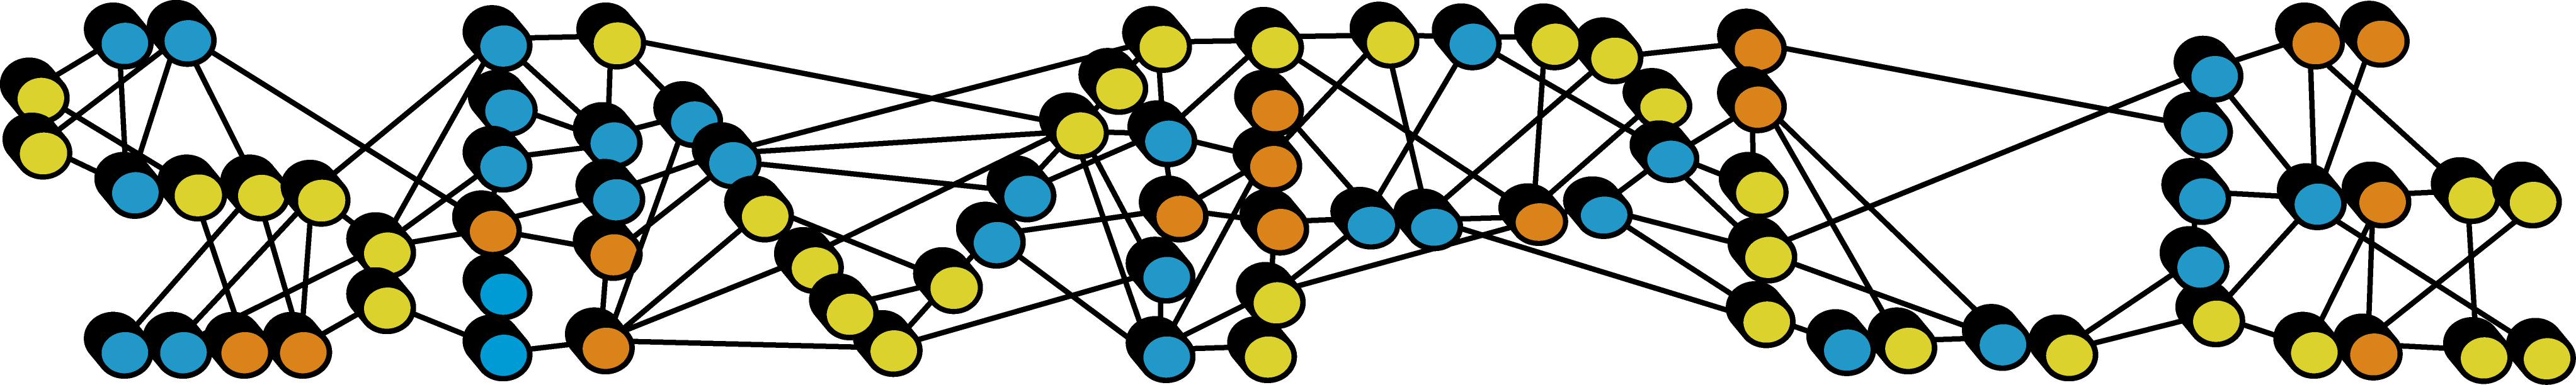
\includegraphics[keepaspectratio=true,scale=0.6]{../SIMPLE_logo/rawlogo}
%\caption{}
\end{figure}

%2do
% Volta phase-plate support

\title{\prgname{The SIMPLE 3.0 Command-line Manual}}
\date{Jan 11, 2019}
\maketitle

\vspace{1em}
\begin{minipage}[ht]{0.50\textwidth}
\textbf{Contributors:}\\
cyril.reboul@monash.edu\\
simon.kiesewetter@monash.edu\\
chiara.machello@monash.edu\\
dominika.elmlund@monash.edu\\
hans.elmlund@monash.edu\\
\textbf{Adress:}\\
Biomedicine Discovery Institute\\
Monash University\\
3800 Clayton, VIC, Australia\\
\textbf{Webpage:}\\
www.simplecryoem.com\\
\textbf{Contact:}\\
\url{http://simplecryoem.com/contact.html}\\
dominika@simplecryoem.com\\
\end{minipage}
\vspace{20pt}

\begin{quote}
\textbf{``Keep it SIMPLE stupid''}\\(\textit{Kelly Johnson}; lead engineer at the Lockheed Skunk Works, coined the famous KISS principle stating that systems work best if they are kept simple rather than made complex. Therefore, simplicity should be a key goal in design and unnecessary complexity should be avoided.)
\end{quote}

\begin{quote}
\textbf{``Everything should be made as SIMPLE as possible, but no SIMPLEr''}\\(\textit{Albert Einstein})
\end{quote}

\begin{quote}
\textbf{``Complex theories do not work, SIMPLE algorithms do''}\\(\textit{Vladimir N. Vapnik}; author of \textit{The Nature of Statistical Learning Theory})
\end{quote}
\clearpage

\tableofcontents{}
\clearpage

\section{About SIMPLE}

\textbf{S}ingle-particle \textbf{IM}age \textbf{P}rocessing \textbf{L}inux \textbf{E}ngine (\href{www.simplecryoem.com}{\textbf{\textcolor{BurntOrange}{SIMPLE}}}) is a program package for cryo-EM image processing, covering all aspects of the single-particle analysis workflow. SIMPLE also provides tools for atomic-resolution 3D reconstruction from time-series of nanoparticles imaged in solution with graphene liquid cell TEM. The SIMPLE back-end consists of an object-oriented numerical library written in modern Fortran. In the latest SIMPLE release (version 3.0), we have revised the way that meta-data and input parameters are handled, providing a project-based execution model (described below). This model has made SIMPLE easier to use, improved output data organisation and increased performance. This document describes the command-line interface of SIMPLE and is intended for advanced users and/or developers that wish to build applications utilising the high-performance image processing algorithms in SIMPLE. <REFERENCE FOR LESS EXPERIENCED USERS>
 
SIMPLE is free software: you can redistribute it and/or modify it under the terms of the \href{http://www.gnu.org/copyleft/gpl.html}{\textbf{\textcolor{BurntOrange}{GNU General Public License}}} as published by the Free Software Foundation, either version 3 of the license, or (at your option) any later version. SIMPLE is distributed with the hope that it will be useful, but WITHOUT ANY WARRANTY; without even the implied warranty of MERCHANTABILITY or FITNESS FOR A PARTICULAR PURPOSE. See the \href{http://www.gnu.org/copyleft/gpl.html}{\textbf{\textcolor{BurntOrange}{GNU General Public License}}} for more details.

\section{Installation instructions}

\subsection{System requirements}
\begin{itemize}
	\item[--] Linux (we use Ubuntu 15.04 and above)
	\item[--] MacOSX: 10.10 and above
	\item[--] CMake 3.2 and above
	\item[--] FFTW 3.3 and above
	\item[--] GNU toolchain (gcc \& gfortran) 4.9 to 5.4
\end{itemize}

\subsection{Installation}
\noindent{}\textbf{Step 1:} Create the directory in which you are going to install SIMPLE (referred to here as \texttt{<simple\_path>})

\begin{Verbatim}[commandchars=+\[\],fontsize=\small,breaklines=true]
mkdir <simple_path>
\end{Verbatim}

\noindent{}\textbf{Step 2:} Unzip the SIMPLE 3.0 tar ball in this directory (assuming you have downloaded the tar ball in the \texttt{<downloads>} directory)

\begin{Verbatim}[commandchars=+\[\],fontsize=\small,breaklines=true]
mv <downloads>/SIMPLE3.0.tgz <simple path>
cd <simple path>
tar -xzf SIMPLE3.0.tgz
\end{Verbatim}

\noindent{}\textbf{Step 3:} Create a directory for the build

\begin{Verbatim}[commandchars=+\[\],fontsize=\small,breaklines=true]
cd simple3.0
mkdir build
cd build
\end{Verbatim}

\noindent{}\textbf{Step 4:} Compile and install SIMPLE 3.0

\begin{Verbatim}[commandchars=+\[\],fontsize=\small,breaklines=true]
cmake ../
make -j install
\end{Verbatim}

\noindent{}This will install SIMPLE in the \texttt{'build'} directory, clean out all unnecessary
files and will finish with the following message (a reminder for step 5 below):

\begin{Verbatim}[commandchars=+\[\],fontsize=\small,breaklines=true]
Installation complete.
==========================================================================
Please ensure the following variables are set properly in add2.*rc file:
    SIMPLE_EMAIL SIMPLE_QSYS SIMPLE_PATH SIMPLE_SOURCE_PATH
To use SIMPLE, append the relevant add2.* to your HOME shell rc file:
  bash$ cat add2.bashrc >> ~/.bashrc
  tcsh$ cat add2.tcshrc >> ~/.tcshrc
==========================================================================
For minimal installation to work correctly add:
<your src path>/Simple-release/build/bin and
<your src path>/Simple-release/build/scripts
to your PATH environment variable.
==========================================================================
\end{Verbatim}

\noindent{}When the build and installation directories are the same (default) and you are
happy with the install, you may want to clean compilation-generated and
unnecessary files using \texttt{distclean}.

\begin{Verbatim}[commandchars=+\[\],fontsize=\small,breaklines=true]
make distclean
\end{Verbatim}

\noindent{}If you wish to provide an alternative installation directory, substitute step 4 with

\begin{Verbatim}[commandchars=+\[\],fontsize=\small,breaklines=true]
cmake -DCMAKE_INSTALL_PREFIX=<alternative directory> ../
make -j install
\end{Verbatim}

\noindent{}Step 4 assumes that gcc/gfortran and FFTW are installed in fairly standard directories on your machine. In case you have a 
more exotic setup you can provide the paths pointing to your custom gcc/gfortran \& FFTW by substituting step 4 with

\begin{Verbatim}[commandchars=+\[\],fontsize=\small,breaklines=true]
FC=<gcc/gfortran path> FFTW_DIR=<FFTW path> cmake ../
make -j install
\end{Verbatim}

\noindent{}For instance, on MacOS:
\begin{itemize}
	\item[--] Macports users may use: FC=/opt/local/bin/gfortran FFTW\_DIR=/opt/local;
	\item[--] Fink users: FC=/sw/bin/gfortran FFTW\_DIR=/sw/; and
	\item[--] Homebrew users: FC=/usr/local/bin/gfortran FFTW\_DIR=/usr/local/
\end{itemize}

\noindent{}\\\textbf{Step 5:} Set the environment variables.

\noindent{}\\To run SIMPLE, the bin and scripts paths need to be in the \texttt{PATH} environment
variable. The \texttt{SIMPLE\_PATH} environment variable must also be defined. The 
shell scripts \texttt{add2.bashrc} and \texttt{add2.tcshrc} containing the necessary
instructions were generated during the build step. For immediate use for running and testing, execute

\begin{Verbatim}[commandchars=+\[\],fontsize=\small,breaklines=true]
source add2.bashrc
\end{Verbatim}

\noindent{}or, for TCSH/CSH users:

\begin{Verbatim}[commandchars=+\[\],fontsize=\small,breaklines=true]
source add2.tcshrc
\end{Verbatim}

\noindent{}For permanent installation \texttt{BASH} users should add the contents of \texttt{add2.bashrc} to your \texttt{<HOME>/.bashrc}

\begin{Verbatim}[commandchars=+\[\],fontsize=\small,breaklines=true]
cat add2.bashrc >> ~/.bashrc
\end{Verbatim}

\noindent{}or for TCSH/CSH users:

\begin{Verbatim}[commandchars=+\[\],fontsize=\small,breaklines=true]
cat add2.tcshrc >> ~/.tcshrc
\end{Verbatim}

\subsection{Testing the build}

\noindent{}To ensure that SIMPLE has been correctly installed, we recommend running the application \texttt{simple\_test\_install}. It will test the most 
important components in the SIMPLE library  (those used by prime2D and  prime3D). Execute

\begin{Verbatim}[commandchars=+\[\],fontsize=\small,breaklines=true]
simple_test_install 
\end{Verbatim}

\noindent{}The program will create its own folder \texttt{SIMPLE\_TEST\_INSTALL*date*} where temporary files and information about each 
test are stored. Upon succesful completion you should see

\begin{Verbatim}[commandchars=+\[\],fontsize=\small,breaklines=true]
 **** SIMPLE_TEST_INSTALL NORMAL STOP ****
\end{Verbatim}

\noindent{}\texttt{simple\_test\_install} can be executed anywhere. After execution, the folder created can be safely removed. If any of the individual 
tests fail an error message will be displayed. If you detect an error, please carefully check the SIMPLE and FFTW installations 
and the gfortran version. If you still have issues, please file a help ticket on the webpage.

\subsection{Installation/configuration on a Linux cluster}

Installation on a Linux cluster is essentially the same as on a Linux workstation with the exception that the appropriate modules need to be loaded before installation and execution. On a typical SLURM cluster
\begin{Verbatim}[commandchars=+\[\],fontsize=\small,breaklines=true]
module load fftw/3.3.4-gcc
module load gcc/4.9.1
\end{Verbatim}
The instructions for how to execute SIMPLE in distributed environments (clusters or workstations with more than one CPU socket) are described below \label{distr}.

\section{What is new in SIMPLE release 3.0?}
The number of changes we have made to the suite compared to the previously released version (2.5) are too many to list here. If you have experience with previous SIMPLE releases, please have a quick browse through the manual. We promise you will catch-up quickly. Most (but not all) of the algorithms implemented in SIMPLE have been published (REFS). If you want to understand the theory, we recommend you read the papers. This document exclusively describes the command-line driven SIMPLE user interface and basic knowledge about EM and single-particle analysis is assumed. 

\subsection{SIMPLE program naming convention}
The first big change you will notice is that all program names have changed to plain English descriptions of their functionality.  For example, \prgname{PRIME2D} that does simultaneous 2D alignment and clustering in a reference-free manner is now called \prgname{cluster2D}, the workflow for \textit{ab initio} 3D reconstruction from class averages is called \prgname{initial\_3Dmodel}, the 3D refinement application is called \prgname{refine3D} and the heterogeneity analysis tool is called \prgname{cluster3D}. In SIMPLE, we distinguish between \textit{distributed workflows} (executed with \texttt{simple\_distr\_exec}) and \textit{programs} (executed with \texttt{simple\_exec}). Programs perform smaller tasks (subjected exclusively to OpenMP-thread-based parallelisation), whereas distributed workflows are major image processing steps that typically require a multi-core workstation or a computer cluster. Finally, there is a third executable \texttt{simple\_private\_exec} that is used internally by SIMPLE, by the SIMPLE developers and by very advanced users that want to test experimental aspects of SIMPLE or use functionality to support building GUI applications on top of SIMPLE.

\subsection{SIMPLE input parameter categorisation}
Another noticeable change is they way the command-line instructions are provided when you execute a SIMPLE program or distributed workflow. For example, this is what is written in the terminal when executing \texttt{simple\_distr\_exec prg=refine3D}
\begin{Verbatim}[commandchars=+\[\],fontsize=\small,breaklines=true]
+underline[USAGE]
+textit[bash-3.2$ simple_distr_exec prg=refine3D key1=val1 key2=val2 ...]
Required input parameters in +textbf[bold] (ensure terminal support)
+underline[IMAGE INPUT/OUTPUT]
vol1 = Reference volume; input volume e.g. vol.mrc
+underline[SEARCH CONTROLS]
+textbf[pgrp         = Point-group symmetry; point-group(cn|dn|t|o|i){c1}]
center       = Center reference volume(s); (yes|no){yes}
continue     = Continue previous refinement; (yes|no){no}
frac         = Fraction of particles to include; fraction of particles(0.1-0.9){1.0}
maxits       = Max iterations; Max # iterations
neigh        = Neighbourhood refinement; (yes|no){no}
nnn          = Number of nearest neighbours; # projection neighbours{10% of search space}
nrestarts    = Number of restarts; # restarts{1}
nspace       = Number of projection directions; # projections
nstates      = Number of states; # states to reconstruct
objfun       = Objective function; (cc|ccres|euclid){cc}
refine       = Refinement mode; (snhc|single|multi|greedy_single|cont_single|greedy_multi|cluster|clustersym){single}
sigma2_fudge = Sigma2-fudge factor; {100.}
trs          = Maximum translational shift; max shift per iteration in pixels{5}
update_frac  = Fractional update per iteration; update this fraction per iter(0.1-0.5){1.0}
+underline[FILTER CONTROLS]
cenlp      = Centering low-pass limit; centering low-pass limit in Angstroms{30}
eo         = Gold-standard FSC for filtering and resolution estimation; (yes|no){no}
hp         = High-pass limit; high-pass limit in Angstroms
lp         = Static low-pass limit; low-pass limit in Angstroms
lplim_crit = Low-pass limit FSC criterion; low-pass FSC criterion(0.143-0.5){0.3}
lpstop     = Low-pass limit for frequency limited refinement; low-pass limit in Angstroms
shellw     = B-factor weighted reconstruction; (yes|no){no}
+underline[MASK CONTROLS]
+textbf[msk      = Mask radius; mask radius in pixels]
focusmsk = Mask radius in focused refinement; focused mask radius in pixels
inner    = Inner mask radius; inner mask radius in pixels
mskfile  = Input mask file; e.g. automask.mrc from postprocess
width    = Falloff of inner mask; # pixels cosine edge{10}
+underline[COMPUTER CONTROLS]
+textbf[nparts = Number of parts; divide job into # parts]
+textbf[nthr   = Number of threads per part, give 0 if unsure; # shared-memory CPU threads]
\end{Verbatim}

\noindent{}The number of input parameters can be daunting and to simplify the representation we have divided them into the following categories.

\begin{itemize}
    \item[--] \textbf{IMAGE INPUT/OUTPUT} consists of MRC format stacks or volumes.
    \item[--] \textbf{PARAMETER INPUT/OUTPUT} are parameters associated with the inputted images.
    \item[--] \textbf{ALTERNATIVE INPUTS} is for programs that accept alternative inputs: volume or stack, for example.
    \item[--] \textbf{SEARCH CONTROLS} are parameters that control optimisation.
    \item[--] \textbf{FILTER CONTROLS} are parameters that control Fourier filtering options.
    \item[--] \textbf{MASK CONTROLS} are parameters that control real-space masking options.
    \item[--] \textbf{COMPUTER CONTROLS} are parameters that specifies how to utilise the computing environment.
\end{itemize}

\noindent{}The required command-line parameters are printed in \textbf{bold}. Hence, the execution of  \texttt{simple\_distr\_exec prg=refine3D} could be as trivial as

\begin{Verbatim}[commandchars=+\[\],fontsize=\small,breaklines=true]
simple_distr_exec prg=refine3D pgrp=c1 msk=120 nparts=4 nthr=8
\end{Verbatim}

\noindent{}We have encapsulated all the details of the SIMPLE user interface in an abstract data type. A JSON description of the SIMPLE user interface can be obtained through 

\begin{Verbatim}[commandchars=+\[\],fontsize=\small,breaklines=true]
simple_private_exec prg=write_ui_json
\end{Verbatim}

\noindent{}This produces the file \texttt{simple\_user\_interface.json} describing all distributed workflows and programs in SIMPLE. This may be useful for building GUI applications on top of the SIMPLE back-end.

\subsection{SIMPLE project execution model}

The final major change that affects SIMPLE usage is the project-based execution model that encapsulates all meta-data in a single file and provides a complete and reversible history of the SIMPLE project. This is best illustrated by example. Below, we provide the commands executed for reconstructing HCN (EMPIAR-10081) to 3.4 A resolution.

\begin{Verbatim}[commandchars=+\[\],fontsize=\small,breaklines=true]
simple_exec prg=new_project projname=hcn_test
\end{Verbatim}

\noindent{}This creates the project, represented by a directory created in the current working directory called \texttt{hcn\_test} and in that directory a binary file called \texttt{hcn\_test.simple} that will be filled up with meta-data as the project progresses. Next, we change directory to the project directory and import some data.

\begin{Verbatim}[commandchars=+\[\],fontsize=\small,breaklines=true]
cd hcn_test
simple_exec prg=import_particles cs=2.7 ctf=yes fraca=0.1 kv=300 smpd=1.3 stk=/media/hael/LongTermStorage/EM-data/HCN/hcn_shiny.mrc deftab=/media/hael/LongTermStorage/EM-data/HCN/deftab.txt
\end{Verbatim}

\noindent{}This imports an MRC stack with associated CTF parameters to the project. If you list the content of the project directory you will see that the directory \texttt{1\_import\_particles} was created, containing a \texttt{hcn\_test.simple} file. What happened here? First, the import program created its execution directory, then made a copy of the project file and in that copy it imported the stack file path and CTF parameter information. The next command is for running a 2D analysis

\begin{Verbatim}[commandchars=+\[\],fontsize=\small,breaklines=true]
nohup simple_distr_exec prg=cluster2D ncls=200 msk=65 nparts=4 nthr=32 > CLS2D &
\end{Verbatim}

\noindent{}By default, SIMPLE looks in the project directory and picks the project file from the execution directory with the highest number as a starting point for the next process. In this example, the 2D analysis picks the project file from the \texttt{1\_import\_particles}. Sometimes you may want to start from another project file and selecting the highest numbered one is not desired. Therefore, the possibility to provide a project file on the command line is given.
\begin{Verbatim}[commandchars=+\[\],fontsize=\small,breaklines=true]
projfile=X_execution_dir/project_file.simple
\end{Verbatim}

\noindent{}If desired, it is also possible to turn off the execution directory generation and run the process straight in the current working directory. This is done by giving

\begin{Verbatim}[commandchars=+\[\],fontsize=\small,breaklines=true]
mkdir=no
\end{Verbatim}

\noindent{}on the command line. In a realistic situation, you would have used \prgname{cleanup2D} in replacement of \prgname{cluster2D} to remove junk and identify good particles. If you have a GUI running on top of the SIMPLE back-end you would then like to report any selections made in the GUI to the project file. Below, we describe how to do this. This data set was already cleaned with RELION, so we proceed using all class averages for initial 3D model production.

\begin{Verbatim}[commandchars=+\[\],fontsize=\small,breaklines=true]
nohup simple_distr_exec prg=initial_3Dmodel pgrp=c4 hp=60 msk=65 nparts=4 nthr=32 > INI3D &
\end{Verbatim}

\noindent{}Finally, we execute the refinement command

\begin{Verbatim}[commandchars=+\[\],fontsize=\small,breaklines=true]
nohup simple_distr_exec prg=refine3D pgrp=c4 frac=0.9 maxits=15 trs=5 update_frac=0.2 eo=yes hp=60 msk=65 nparts=4 nthr=32 > REFINE3D &
\end{Verbatim}

\noindent{}The final and intermittent results are neatly organised in directories in the project directory

\begin{Verbatim}[commandchars=+\[\],fontsize=\small,breaklines=true]
ls
1_import_particles  3_initial_3Dmodel  CLS2D            INI3D     stack_parts
2_cluster2D         4_refine3D         hcn_test.simple  REFINE3D
\end{Verbatim}

\noindent{}and it is possible to go back to any point in the project history to re-run a job with different parameters or try a different algorithm for the task. Now, let's look closer at the project file.

\subsection{Structure, interrogation and manipulation of the binary project file}
In SIMPLE v3.0 we have implemented an abstract data type called sp\_project that manages all meta-data generated throughout a single-particle analysis project. The multi-segment binary project file is simply a mirror of this data type on disk. Segments 1-10 are reserved  for simple program outputs, orientations and files. Currently implemented segments are

\begin{enumerate}
    \item micrographs
    \item per-micrograph stacks
    \item per-particle 2D orientations
    \item per-cluster 2D orientations
    \item per-cluster 3D orientations
    \item per-particle 3D orientations
    \item critical project outputs
\end{enumerate}

\noindent{}Segments 11-20 are reserved for project info, job management etc. Currently implemented segments are

\begin{enumerate}
   \setcounter{enumi}{10}
    \item project information
    \item command lines of processes executed
    \item computing environment specification
\end{enumerate}

\noindent{}All of these segments utilise the SIMPLE orientation container object for data storage and we therefore refer to the different segment types as ``oritype'' with shorthand descriptors

\begin{enumerate}
    \item micrographs, \tab{}\texttt{oritype = \textbf{mic}}
    \item per-micrograph stacks, \tab{}\texttt{oritype = \textbf{stk}}
    \item per-particle 2D orientations, \tab{}\texttt{oritype = \textbf{ptcl2D}}
    \item per-cluster 2D orientations, \tab{}\texttt{oritype = \textbf{cls2D}}
    \item per-cluster 3D orientations, \tab{}\texttt{oritype = \textbf{cls3D}}
    \item per-particle 3D orientations, \tab{}\texttt{oritype = \textbf{ptcl3D}}
    \item critical project outputs,\tab{}\texttt{oritype = \textbf{out}}
\end{enumerate}

\begin{enumerate}
   \setcounter{enumi}{10}
    \item project information, \tab{}\texttt{oritype = \textbf{projinfo}}
    \item command lines of processes executed, \tab{}\texttt{oritype = \textbf{jobproc}}
    \item computing environment specification, \tab{}\texttt{oritype = \textbf{compenv}}
\end{enumerate}

\noindent{}The first method of choice for interrogating the project file is

\begin{Verbatim}[commandchars=+\[\],fontsize=\small,breaklines=true]
simple_exec prg=print_project_info
\end{Verbatim}

\noindent{}Going back to out HCN example, we cd to the \texttt{hcn\_test/4\_refine3D} execution directory and execute \texttt{simple\_exec prg=print\_project\_info}. This produces the output
\begin{Verbatim}[commandchars=+\[\],fontsize=\small,breaklines=true]
+underline[+textbf[SEGMENT 02 of type: stk]]
+textit[4 record(s) of stack (extracted particles) info, one per stack of particles]
+textbf[first record:] stk=../stack_parts/stack_part1.mrc stkkind=split imgkind=ptcl phaseplate=no ctf=yes box=256.000000 nptcls=13968.0000 fromp=1.00000000 top=13968.0000 smpd=1.29999995 kv=300.000000 cs=2.70000005 fraca=0.100000001 state=1.00000000
+underline[+textbf[SEGMENT 03 of type: ptcl2D]]
+textit[55870 record(s) of 2D information generated by cluster2D, one per particle]
+textbf[first record:] kv=300.000000 cs=2.70000005 fraca=0.100000001 dfx=4.13821840 dfy=4.34016752 angast=11.1103058 state=1.00000000 eo=0.00000000 stkind=1.00000000 x=-1.87167823 y=-3.53704500 updatecnt=18.0000000 w=1.00000000 bfac_rec=0.00000000 lp=7.16521692 e3=280.975616 inpl=37.0000000 class=128.000000 corr=0.342293173 specscore=0.198325723 bfac=514.059692 dist_inpl=0.00000000 mi_class=1.00000000 frac=100.000000 e1=0.00000000 e2=0.00000000
+underline[+textbf[SEGMENT 04 of type: cls2D]]
+textit[200 record(s) of data generated by cluster2D, one per 2D cluster]
+textbf[first record:] class=1.00000000 pop=254.000000 res=7.53409100 corr=0.340087920 w=1.00000000 specscore=0.242327988 state=1.00000000
+underline[+textbf[SEGMENT 05 of type: cls3D]]
+textit[200 record(s) of 3D information for class averages, one per class]
+textbf[first record:] dfx=0.00000000 dfy=0.00000000 angast=0.00000000 state=1.00000000 x=-1.16237819 y=-1.83902657 e1=12.5358458 e2=158.906311 e3=305.373138 proj=2409.00000 w=1.00000000 bfac=23.9044113 mi_proj=1.00000000 mi_state=1.00000000 dist=6.78878576E-02 dist_inpl=0.00000000 frac=100.000000 corr=0.943886340 specscore=0.941106677 inpl=1.00000000 spread=0.986059248 shwmean=0.169503510 shwstdev=7.38897547E-02 npeaks=11.0000000 updatecnt=23.0000000 ow=0.173722118 class=1.00000000 lp=10.1947365 stkind=1.00000000
+underline[+textbf[SEGMENT 06 of type: ptcl3D]]
+textit[55870 record(s) of 3D information, one per particle]
+textbf[first record:] kv=300.000000 cs=2.70000005 fraca=0.100000001 dfx=4.13821840 dfy=4.34016752 angast=11.1103058 state=1.00000000 eo=0.00000000 stkind=1.00000000 x=-2.17266393 y=-3.59118795 w=0.00000000 bfac_rec=0.00000000 lp=3.52181816 e3=300.895508 inpl=2.00000000 class=128.000000 corr=0.106535442 specscore=6.47827759E-02 bfac=143.173950 dist_inpl=0.895474195 mi_class=1.00000000 frac=100.000000 e1=1.58313191 e2=92.8490295 proj=1295.00000 updatecnt=3.00000000 dist=2.52782822 ow=2.80490033E-02 spread=3.31418705 shwmean=0.493733585 shwstdev=0.237732679 npeaks=74.0000000 mi_proj=0.857142866
+underline[+textbf[SEGMENT 07 of type: out]]
+textit[6 record(s) of crtitical project outputs: class averages, 3D volumes, FSC/FRC files etc.]
+textbf[first record:] frcs=../2_cluster2D/frcs.bin imgkind=frc2D
+underline[+textbf[SEGMENT 11 of type: projinfo]]
+textit[1 record(s) of information about the project, project name etc.]
+textbf[first record:] projname=hcn_test projfile=hcn_test.simple cwd=/Processing/HCN/hcn_test
+underline[+textbf[SEGMENT 12 of type: jobproc]]
+textit[4 record(s) of all command-lines executed throughout the project]
+textbf[first record:] prg=import_particles ctf=yes stk=/media/hael/LongTermStorage/EM-data/HCN/hcn_shiny.mrc deftab=/media/hael/LongTermStorage/EM-data/HCN/deftab.txt mkdir=yes projfile=/Processing/HCN/hcn_test/1_import_particles/hcn_test.simple projname=hcn_test exec_dir=1_import_particles date=20190104.0 time=161342.797 cs=2.70000005 fraca=0.100000001 kv=300.000000 smpd=1.29999995
+underline[+textbf[SEGMENT 13 of type: compenv]]
+textit[1 record(s) of computing environment specifications, queue system, memory per job etc.]
+textbf[first record:] simple_path=/home/hael/src/SIMPLE3.0/build qsys_name=local user_email=my.name@uni.edu job_name=simple_hcn_test time_per_image=100.000000 job_memory_per_task=16000.0000
\end{Verbatim}

\noindent{}You notice that what happened in the HCN workflow is directly reflected in the project file structure. The \prgname{cluster2D} analysis split the imported stack into four parts (one per partition used), which is why the \texttt{\textbf{stk}} segment contains 4 records. The first record of the segment is also printed and we see that the first record of the \texttt{\textbf{stk}} segment contains the filename in addition to a number of parameters associated with the stack file, represented by key-value entries. Next, the \prgname{cluster2D} analysis filled-in the \texttt{\textbf{ptcl2D}} segment with 55870 records (one per particle) and the \texttt{\textbf{cls2D}} segment with 200 records (one per class). Subsequently, the \prgname{initial\_3Dmodel} workflow provided 200 records in the \texttt{\textbf{cls3D}} segment, describing class average orientations. Finally, the  \prgname{refine3D} workflow provided 55870 records of 3D orientations and various other statistics (one per particle) in the \prgname{ptcl3D} segment. There are 7 records of critical project outputs in the \texttt{\textbf{out}} segment (SEGMENT 07) and to inspect them closer we use the following command

\begin{Verbatim}[commandchars=+\[\],fontsize=\small,breaklines=true]
simple_exec prg=print_project_field oritype=out
\end{Verbatim}

\noindent{}This produces the output

\begin{Verbatim}[commandchars=+\[\],fontsize=\small,breaklines=true]
frcs=../2_cluster2D/frcs.bin imgkind=frc2D
stk=../2_cluster2D/cavgs_iter018.mrc stkkind=single imgkind=cavg ctf=no box=256.000000 nptcls=200.000000 fromp=1.00000000 top=200.000000 smpd=1.29999995
vol=../3_initial_3Dmodel/rec_final.mrc imgkind=vol_cavg box=256.000000 smpd=1.29999995 state=1.00000000
fsc=../4_refine3D/fsc_state01.bin imgkind=fsc state=1.00000000 box=256.000000
vol=../4_refine3D/aniso_optlp_state01.mrc imgkind=vol_filt box=256.000000 smpd=1.29999995 state=1.00000000
vol=../4_refine3D/recvol_state01_iter015.mrc imgkind=vol box=256.000000 smpd=1.29999995 state=1.00000000
\end{Verbatim}

\noindent{}\prgname{cluster2D} provided two critical outputs: a file of Fourier Ring Correlations (\texttt{frcs}) and a stack of class averages (\texttt{stk}). \prgname{initial\_3Dmodel} provided one volume output. Finally, \prgname{refine3D} provided three outputs: Fourier Shell Correlations (\texttt{fsc}) and two volumes. 

\section{File formats}

\subsection{Image file formats}
SIMPLE supports SPIDER (\texttt{*.spi}) and MRC (\texttt{*.mrc}) formats for image stacks and volumes. The MRC file handling classes are shared with the the FREALIX program for helical reconstruction \citep{Rohou:2014aa}. RELION \citep{Scheres:2012aa} uses the convention that MRC stacks have the suffix \texttt{*.mrcs} and volumes the suffix \texttt{*.mrc}. This is to overcome the annoyance that it is not possible to tell from an MRC file header whether a MRC file is a volume or a stack. With SIMPLE you can select to use either the \texttt{*.mrcs} or \texttt{*.mrc} suffix for stacks. The way that we keep track of whether a file is a volume or stack is via the command line key value. The key-value pairs \texttt{vol1=rec.mrc} and \texttt{vol2=rec2.mrc} refer to volumes whereas the key-value pairs \texttt{stk=ptcls.mrc} and \texttt{stk2=ptcls2.mrc} refer to stacks.

\subsection{SIMPLE parameter file format}
The SIMPLE text-files used for parameter input/output use a \texttt{key=value} syntax of the form
\begin{Verbatim}[commandchars=+\[\],fontsize=\small,breaklines=true]
e1=80. e2=100. e3=5.5 x=1.23 y=4.25 dfx=2.56 dfy=2.54 angast=30.5 state=1
\end{Verbatim}
to represent per-particle information. Internally, the orientation information is stored in a dynamic hash data structure, which gives the file format high flexibility. Therefore, writing conversion scripts to allow interchange of parameters between SIMPLE and other packages is easy. SIMPLE uses the same conventions as FREALIGN \citep{Grigorieff:2007aa} to represent orientations and CTF parameters. The CTF parameterisation obtained by CTFFIND \citep{Mindell:2003aa} can be directly plugged into SIMPLE, for example by creating a file \texttt{deftab.txt}, looking like
\begin{Verbatim}[commandchars=+\[\],fontsize=\small,breaklines=true]
dfx=2.56 dfy=2.76 angast=30.5
dfx=3.50 dfy=3.33 angast=60.0
dfx=1.98 dfy=2.02 angast=120.5
...
\end{Verbatim}
It is also possible to import data using plain text files, as described below.

\subsection{Parameter File Conversions}
The \texttt{SIMPLE/scripts} folder contains perl-scripts (\texttt{convert\_frealign2simple.pl}) and\\ (\texttt{convert\_relion2simple.pl}) to convert FREALIGN and RELION parameter files, respectively, file to a SIMPLE parameter file. This is easy, since these software packages internally use the \href{http://spider.wadsworth.org/spider_doc/spider/docs/euler.html}{\textbf{\textcolor{BurntOrange}{Spider Euler angle convention}}}. Other packages may use other conventions. There's also a \texttt{relion2emanbox.pl} script for converting box files obtained with RELION to the EMAN \texttt{*.box} format used by SIMPLE.



\section{SIMPLE usage}

\subsection{SIMPLE help tools}
In attempt to reduce the dependency on the manual, we have packaged a lot of the documentation in the software itself. For example
\begin{Verbatim}[commandchars=+\[\],fontsize=\small,breaklines=true]
simple_exec prg=list
center
cluster_cavgs
convert
ctfops
export_starproject
extract
filter
fsc
info_image
info_stktab
import_boxes
...
\end{Verbatim}
lists all programs executed with \texttt{simple\_exec} (shared-memory parallelisation) and
\begin{Verbatim}[commandchars=+\[\],fontsize=\small,breaklines=true]
simple_distr_exec prg=list
cleanup2D
cluster2D
cluster2D_stream
cluster3D
cluster3D_refine
ctf_estimate
gen_pspecs_and_thumbs
initial_3Dmodel
make_cavgs
motion_correct
motion_correct_tomo
pick
pick_extract_stream
preprocess
preprocess_stream
reconstruct3D
refine3D
refine3D_init
scale_project
tseries_track
\end{Verbatim}
lists all distributed workflows executed with \texttt{simple\_distr\_exec}. If you don't quite remember which program you are looking for but remember that it was called \texttt{cluster} something, you could execute
\begin{Verbatim}[commandchars=+\[\],fontsize=\small,breaklines=true]
simple_distr_exec prg=list | grep cluster
cluster2D
cluster2D_stream
cluster3D
cluster3D_refine
\end{Verbatim}
If you want a description for a particular program, for example \prgname{cluster2D}, execute
\begin{Verbatim}[commandchars=+\[\],fontsize=\small,breaklines=true]
simple_distr_exec prg=cluster2D describe=yes
is a distributed workflow implementing a reference-free 2D alignment/clustering algorithm adopted from the prime3D probabilistic ab initio 3D reconstruction algorithm
\end{Verbatim}
To obtain a description of the what command line options are available, execute
\begin{Verbatim}[commandchars=+\[\],fontsize=\small,breaklines=true]
simple_distr_exec prg=cluster2D
\end{Verbatim}

\subsection{SIMPLE distributed workflows, categorisation and description}

\subsubsection{PRE-PROCESSING WORKFLOWS}
\begin{itemize}
\item[--] \prgname{preprocess} is a distributed workflow that executes \prgname{motion\_correct}, \prgname{ctf\_estimate} and \prgname{pick} in sequence
\item[--] \prgname{preprocess\_stream} is a distributed workflow that executes \prgname{motion\_correct}, \prgname{ctf\_estimate} and \prgname{pick} in streaming mode as the microscope collects the data
\item[--] \prgname{motion\_correct} is a distributed workflow for motion correction of movies based on the same principal strategy as Grigorieff's program. There are two important differences: automatic weighting of the frames using a correlation-based M-estimator and continuous optimisation of the shift parameters. If dose\_rate and exp\_time are given the individual frames will be low-pass filtered accordingly (dose-weighting strategy). If scale is given, the movie will be Fourier cropped according to the down-scaling factor (for super-resolution movies). If nframesgrp is given the frames will be pre-averaged in the given chunk size (Falcon 3 movies). If fromf/tof are given, a contiguous subset of frames will be averaged without any dose-weighting applied
\item[--] \prgname{gen\_pspecs\_and\_thumbs} is a distributed workflow for generating power spectra and thumbnails for imported integrated movies
\item[--] \prgname{motion\_correct\_tomo} is a distributed workflow for motion correction of movies based on the same principal strategy as Grigorieff's program. There are two important differences: automatic weighting of the frames using a correlation-based M-estimator and continuous optimisation of the shift parameters. If dose\_rate and exp\_time are given the individual frames will be low-pass filtered accordingly (dose-weighting strategy). The exp\_doc document should contain per line \texttt{exp\_time=X} and \texttt{dose\_rate=Y}. It is assumed that the input list of movies (one per tilt) are ordered temporally. This is necessary for correct dose-weighting of tomographic tilt series. If scale is given, the movie will be Fourier cropped according to the down-scaling factor (for super-resolution movies). If \texttt{nframesgrp} is given the frames will be pre-averaged in the given chunk size (Falcon 3 movies)
\item[--] \prgname{ctf\_estimate} is a distributed SIMPLE workflow for CTF parameter fitting
\item[--] \prgname{pick} is a distributed workflow for template-based particle picking
\item[--] \prgname{pick\_extract\_stream} is a distributed workflow for template-based particle picking and extraction in streaming mode
\end{itemize}

\subsubsection{CLUSTER2D WORKFLOWS}
\begin{itemize}
\item[--] \prgname{make\_cavgs} is a distributed workflow for generating class averages or initial random references for \prgname{cluster2D} execution
\item[--] \prgname{cleanup2D} is a distributed workflow implementing a reference-free 2D alignment/clustering algorithm suitable for the first pass of cleanup after picking
\item[--] \prgname{cluster2D} is a distributed workflow implementing a reference-free 2D alignment/clustering algorithm adopted from the prime3D probabilistic ab initio 3D reconstruction algorithm
\item[--] \prgname{cluster2D\_stream} is a distributed workflow implementing \prgname{cluster2D} in streaming mode
\end{itemize}

\subsubsection{AB INITIO 3D RECONSTRUCTION WORKFLOW}
\begin{itemize}
\item[--] \prgname{initial\_3Dmodel} is a distributed workflow for generating an initial 3D model from class averages obtained with \prgname{cluster2D}
\end{itemize}

\subsubsection{REFINE3D WORKFLOWS}
\begin{itemize}
\item[--] \prgname{refine3D\_init} is a distributed workflow for generating a random initial 3D model for initialisation of \prgname{refine3D}
\item[--] \prgname{refine3D} is a distributed workflow for 3D refinement based on probabilistic projection matching
\item[--] \prgname{reconstruct3D} is a distributed workflow for reconstructing volumes from MRC and SPIDER stacks, given input orientations and state assignments. The algorithm is based on direct Fourier inversion with a Kaiser-Bessel (KB) interpolation kernel
\end{itemize}

\subsubsection{CLUSTER3D WORKFLOWS}
\begin{itemize}
\item[--] \prgname{cluster3D} is a distributed workflow for heterogeneity analysis by 3D clustering
\item[--] \prgname{cluster3D\_refine} is a distributed workflow based on probabilistic projection matching for refinement of 3D heterogeneity analysis by \prgname{cluster3D}
\end{itemize}

\subsubsection{TIME-SERIES WORKFLOWS}
\begin{itemize}
\item[--] \prgname{tseries\_track} is a distributed workflow for particle tracking in time-series data
\end{itemize}

\subsubsection{MISCELLANEOUS WORKFLOWS}
\begin{itemize}
\item[--] \prgname{scale\_project} is a distributed workflow for re-scaling MRC \& SPIDER stacks part of project specification
\end{itemize}

\subsection{SIMPLE programs, categorisation and description of }

\subsubsection{PROJECT MANAGEMENT PROGRAMS}
\begin{itemize}
\item[--] \prgname{new\_project} is a program for creating a new project. SIMPLE3.0 relies on a monolithic project file for controlling execution on distributed and shared-memory systems and for unified meta-data management. This program creates a directory named projname and a file projname.simple inside that directory that contains all information about the project as well as all meta data generated by the different SIMPLE programs. This file is mirrored by an abstract data type in the back-end, which manages the parameters and meta-data I/O required for execution of SIMPLE
\item[--] \prgname{update\_project} is a program for updating an existing project: changing the name/user\_email/ computer controls
\item[--] \prgname{print\_project\_info} is a program prints information about a *.simple project file
\item[--] \prgname{print\_project\_field} is a program for printing an orientation field in the project data structure (segment in *.simple project file)
\item[--] \prgname{import\_movies} is a program for importing DDD movies to the project. The movies can be located in any read-only location accessible to the project. If the movies contain only a single frame, they will be interpreted as motion-corrected and integrated. Box files (in EMAN1.9 format) can be imported along with the movies
\item[--] \prgname{import\_boxes} is a program for importing EMAN1.9 box coordinates to the project. The *box (text) files should be listed in boxtab
\item[--] \prgname{import\_particles} is a program for importing extracted particle images to the project
\item[--] \prgname{import\_cavgs} is a program for importing class averages movies to the project
\item[--] \prgname{subset\_project} is a program that generates a random subset of an existing project
\item[--] \prgname{export\_starproject} is a program for exporting a SIMPLE project as a STAR-formatted EM project
\item[--] \prgname{import\_starproject} is a program for importing STAR-formatted EM project files to the current SIMPLE project and saving as a SIMPLE project
\item[--] \prgname{report\_selection} is a program for reporting external (GUI) selections to the SIMPLE project
\end{itemize}

\subsubsection{SINGLE-PARTICLE WORKFLOW PROGRAMS}
\begin{itemize}
\item[--] \prgname{extract} is a program for extracting particle images from integrated movies
\item[--] \prgname{reextract} is a program for re-extracting particle images from integrated movies based on determined 2D/3D shifts
\item[--] \prgname{cluster\_cavgs} is a program for analyzing class averages with affinity propagation, in order to get a better understanding of the view distribution. The balance flag is used to apply a balancing restraint (on the class population). Adjust balance until you are satisfied with the shape of the histogram
\item[--] \prgname{symaxis\_search} is a program for searching for the principal symmetry axis of a volume reconstructed in C1. The rotational transformation is applied to the oritype field in the project and the project file is updated. If you are unsure about the point-group, use the \prgname{symmetry\_test} program instead
\item[--] \prgname{symmetry\_test} is a program that implements a statistical test for point-group symmetry. Input is a volume reconstructed without symmetry (c1) and output is the most likely point-group symmetry
\item[--] \prgname{postprocess} is a program for map post-processing. Use program volops to estimate the B-factor with the Guinier plot
\end{itemize}

\subsubsection{IMAGE PROCESSING PROGRAMS}
\begin{itemize}
\item[--] \prgname{mask} is a program for masking of 2D images and volumes. If you want to mask your images with a spherical mask with a soft  falloff, set msk to the radius in pixels
\item[--] \prgname{fsc} is a program for calculating the FSC between the two input volumes
\item[--] \prgname{local\_resolution} is a program for estimating local resolution based on neighbourhood correlation analysis in e/o maps
\item[--] \prgname{local\_resolution2D} is a program for estimating local resolution based on neighbourhood correlation analysis in e/o cavgs
\item[--] \prgname{center} is a program for centering a volume and mapping the shift parameters back to the particle images
\item[--] \prgname{reproject} is a program for re-projecting a volume using Fourier interpolation. Input is a SPIDER or MRC volume. Output is a stack of projection images of the same format as the inputted volume. Projections are generated by extracting central sections from the Fourier volume and back transforming the 2D FTs. nspace controls the number of projection directions. The  oritab parameter allows you to input the orientations that you wish to have your volume projected in. pgrp controls the point-group symmetry c (rotational), d (dihedral), t (tetrahedral), o (octahedral) or i (icosahedral). The point-group symmetry is used to restrict the set of projections to within the asymmetric unit. neg inverts the contrast of the projections
\item[--] \prgname{volops} is a program that provides standard single-particle image processing routines for MRC or SPIDER volumes
\item[--] \prgname{convert} is a program for converting between SPIDER and MRC formats
\item[--] \prgname{ctfops} is a program for applying CTF to stacked images
\item[--] \prgname{filter} is a program for filtering stack/volume
\item[--] \prgname{normalize} is a program for normalization of MRC or SPIDER stacks and volumes
\item[--] \prgname{scale} is a program for re-scaling, clipping and padding MRC \& SPIDER stacks and volumes
\item[--] \prgname{stack} is a program for stacking individual images (list) or multiple stacks into one
\item[--] \prgname{stackops} is a program that provides standard single-particle image processing routines for MRC or SPIDER stacks. To extract a particular state, give \texttt{oritab} and set \texttt{state}. To select the fraction of best particles, give \texttt{oritab} and set frac. State and frac options can be combined. To apply noise, give the desired signal-to-noise ratio via snr. To calculate the autocorrelation function, set acf=yes. To extract a contiguous subset of images from the stack, set fromp and top. To extract a number of particle images at random, set nran to the desired number. With avg=yes the global average of the stack is calculated. If nframesgrp is set to some integer number >1, averages with chunk sizes of nframesgrp are produced, which may be useful for analysis of dose-fractionated image series. neg inverts the contrast of the images
\item[--] \prgname{shift} is a program for shifting a stack according to origin shifts in oritab
\end{itemize}

\subsubsection{ORIENTATION PROCESSING PROGRAMS}
\begin{itemize}
\item[--] \prgname{make\_oris} is a program for making SIMPLE orientation files. Random Euler angles and random origin shifts are generated. If ndiscrete is set to an integer number > 0, the orientations produced are randomly sampled from the set of ndiscrete quasi-even projection directions, and the in-plane parameters are assigned randomly. If even is set to yes, then all nptcls orientations are assigned quasi-even projection directions and  random in-plane parameters. If nstates is set to some integer number > 0, then states are assigned randomly
\item[--] \prgname{orisops} is a program for modifying SIMPLE orientation/parameter files. If errify=yes, uniform random angular errors, and uniform origin shift errors,  and uniform random defocus errors are introduced. If nstates > 1 then random states are assigned. If mirr=2d, then the Euler angles in oritab are mirrored according to the relation e1=e1, e2=180+e2, e3=-e3. If mirr=3d, then the Euler angles in oritab are mirrored according to the relation R=M(M*R), where R is the rotation matrix calculated from the Euler angle triplet and M is a 3D reflection matrix. If e1, e2, or e3 is inputted, the orientations are rotated correspondingly. If you input state, only the orientations assigned to state state are rotated. If mul is defined, the origin shifts are multiplied with mul. If zero=yes, then the shifts are zeroed
\item[--] \prgname{oristats} is a program for analyzing SIMPLE orientation/parameter files. If two orientation tables (oritab and oritab2) are inputted, statistics of the distances between the orientations in the two documents are provided
\item[--] \prgname{vizoris} is a program for extracting projection directions from orientations for visualization in UCSF Chimera
\end{itemize}

\subsubsection{PRINT INFO PROGRAMS}
\begin{itemize}
\item[--] \prgname{info\_image} is a program for printing header information in MRC and SPIDER stacks and volumes
\item[--] \prgname{info\_stktab} is a program for printing information about stktab (list of stacks)
\item[--] \prgname{print\_fsc} is a program for printing the binary FSC files produced by \prgname{refine3D}
\item[--] \prgname{print\_magic\_boxes} is a program for printing magic box sizes (fast FFT)
\end{itemize}

\subsubsection{SIMULATOR PROGRAMS}
\begin{itemize}
\item[--] \prgname{simulate\_noise} is a program for generating pure noise images
\item[--] \prgname{simulate\_particles} is a program for simulating single-particle cryo-EM images. It is not a very sophisticated simulator, but it is nevertheless useful for testing purposes. It does not do any multi-slice simulation and it cannot be used for simulating molecules containing heavy atoms. It does not even accept a PDB file as an input. Input is a cryo-EM map, which we usually generate from a PDB file using EMANs program pdb2mrc. The volume is projected using Fourier interpolation, 20\% of the total noise is added to the images (pink noise), they are then Fourier transformed and multiplied with astigmatic CTF and B-factor. Next, the they are inverse FTed before the remaining 80\% of the noise (white noise) is added
\item[--] \prgname{simulate\_movie} is a program for crude simulation of a DDD movie. Input is a set of projection images to place. Movie frames are then generated related by randomly shifting the base image and applying noise
\item[--] \prgname{simulate\_subtomogram} is a program for crude simulation of a subtomogram
\end{itemize}

\subsubsection{SYSTEM INTERACTION PROGRAMS}
\begin{itemize}
\item[--] \prgname{mkdir} is a program for making an automatically numbered directory
\end{itemize}

\section{Command line instructions for SIMPLE programs and distributed workflows in alphabetical order}

\subsection{center}
\label{center}
\prgname{center} is a program for centering a volume and mapping the shift parameters back to the particle images, executed by simple\_exec
\begin{Verbatim}[commandchars=+\[\],fontsize=\small,breaklines=true]
+underline[USAGE]
+textit[bash-3.2$ simple_exec prg=center key1=val1 key2=val2 ...]
Required input parameters in +textbf[bold] (ensure terminal support)
+underline[IMAGE INPUT/OUTPUT]
+textbf[vol1 = Volume; input volume e.g. vol.mrc]
+underline[PARAMETER INPUT/OUTPUT]
+textbf[smpd    = Sampling distance; pixel size in Angstroms]
oritab  = Orientation and CTF parameter file; .simple|.txt parameter file
outfile = Output orientation and CTF parameter file; .simple|.txt parameter file
+underline[FILTER CONTROLS]
cenlp = Centering low-pass limit; centering low-pass limit in Angstroms{30}
+underline[COMPUTER CONTROLS]
+textbf[nthr = Number of threads per part, give 0 if unsure; # shared-memory CPU threads]
\end{Verbatim}

\subsection{cleanup2D}
\label{cleanup2D}
\prgname{cleanup2D} is a distributed workflow implementing a reference-free 2D alignment/clustering algorithm suitable for the first pass of cleanup after picking, executed by simple\_distr\_exec
\begin{Verbatim}[commandchars=+\[\],fontsize=\small,breaklines=true]
+underline[USAGE]
+textit[bash-3.2$ simple_distr_exec prg=cleanup2D key1=val1 key2=val2 ...]
Required input parameters in +textbf[bold] (ensure terminal support)
+underline[SEARCH CONTROLS]
+textbf[ncls        = Number of 2D clusters; # 2D clusters]
center      = Center class averages; (yes|no){no}
maxits      = Max iterations; Max # iterations
objfun      = Objective function; (cc|ccres){cc}
update_frac = Fractional update per iteration; update this fraction per iter(0.1-0.5){1.0}
+underline[FILTER CONTROLS]
cenlp = Centering low-pass limit; centering low-pass limit in Angstroms{30}
hp    = High-pass limit; high-pass limit in Angstroms
lp    = Static low-pass limit; low-pass limit in Angstroms
+underline[MASK CONTROLS]
msk = Mask radius; mask radius in pixels
+underline[COMPUTER CONTROLS]
+textbf[nparts = Number of parts; divide job into # parts]
+textbf[nthr   = Number of threads per part, give 0 if unsure; # shared-memory CPU threads]
\end{Verbatim}

\subsection{cluster2D}
\label{cluster2D}
\prgname{cluster2D} is a distributed workflow implementing a reference-free 2D alignment/clustering algorithm adopted from the prime3D probabilistic ab initio 3D reconstruction algorithm, executed by simple\_distr\_exec
\begin{Verbatim}[commandchars=+\[\],fontsize=\small,breaklines=true]
+underline[USAGE]
+textit[bash-3.2$ simple_distr_exec prg=cluster2D key1=val1 key2=val2 ...]
Required input parameters in +textbf[bold] (ensure terminal support)
+underline[IMAGE INPUT/OUTPUT]
refs = Initial references; xxx.mrc file with references
+underline[SEARCH CONTROLS]
+textbf[ncls        = Number of 2D clusters; # 2D clusters]
autoscale   = Automatic down-scaling; (yes|no){yes}
bfac        = Correlation B-factor; B-factor in Angstroms^2(>0.0){200}
center      = Center class averages; (yes|no){yes}
frac        = Fraction of particles to include; fraction of particles(0.1-0.9){1.0}
maxits      = Max iterations; Max # iterations
nrestarts   = Number of restarts; # restarts{1}
objfun      = Objective function; (cc|ccres){cc}
refine      = Refinement mode; (snhc|greedy){snhc}
startit     = First iteration; start iterations from here
trs         = Maximum translational shift; max shift per iteration in pixels{5}
update_frac = Fractional update per iteration; update this fraction per iter(0.1-0.5){1.0}
+underline[FILTER CONTROLS]
cenlp      = Centering low-pass limit; centering low-pass limit in Angstroms{30}
hp         = High-pass limit; high-pass limit in Angstroms
locres     = Iterative local resolution estimation and filtering in last phase; (yes|no){no}
lp         = Static low-pass limit; low-pass limit in Angstroms
lpstart    = Initial low-pass limit; initial low-pass limit in Angstroms
lpstop     = Final low-pass limit; final low-pass limit in Angstroms
match_filt = Matched filter; (yes|no){yes}
shellw     = B-factor weighted reconstruction; (yes|no){no}
+underline[MASK CONTROLS]
+textbf[msk   = Mask radius; mask radius in pixels]
inner = Inner mask radius; inner mask radius in pixels
+underline[COMPUTER CONTROLS]
+textbf[nparts = Number of parts; divide job into # parts]
+textbf[nthr   = Number of threads per part, give 0 if unsure; # shared-memory CPU threads]
\end{Verbatim}

\subsection{cluster2D\_stream}
\label{cluster2D_stream}
\prgname{cluster2D\_stream} is a distributed workflow implementing cluster2D in streaming mode, executed by simple\_distr\_exec
\begin{Verbatim}[commandchars=+\[\],fontsize=\small,breaklines=true]
+underline[USAGE]
+textit[bash-3.2$ simple_distr_exec prg=cluster2D_stream key1=val1 key2=val2 ...]
Required input parameters in +textbf[bold] (ensure terminal support)
+underline[PARAMETER INPUT/OUTPUT]
+textbf[dir_target = Target directory; e.g. 1_preprocess_stream]
+underline[SEARCH CONTROLS]
+textbf[ncls           = Number of 2D clusters; # 2D clusters]
+textbf[ncls_start     = Starting number of clusters; initial # clusters]
+textbf[nptcls_per_cls = Particles per cluster; # particles per cluster]
autoscale      = Automatic down-scaling; (yes|no){yes}
center         = Center class averages; (yes|no){no}
lpthresh       = Resolution rejection threshold; Resolution rejection threshold in angstroms{30}
objfun         = Objective function; (cc|ccres){cc}
remap_cls      = Whether to remap 2D clusters; (yes|no){no}
+underline[FILTER CONTROLS]
cenlp      = Centering low-pass limit; centering low-pass limit in Angstroms{30}
hp         = High-pass limit; high-pass limit in Angstroms
lp         = Static low-pass limit; low-pass limit in Angstroms
match_filt = Matched filter; (yes|no){no}
+underline[MASK CONTROLS]
+textbf[msk   = Mask radius; mask radius in pixels]
inner = Inner mask radius; inner mask radius in pixels
+underline[COMPUTER CONTROLS]
+textbf[nparts = Number of parts; divide job into # parts]
+textbf[nthr   = Number of threads per part, give 0 if unsure; # shared-memory CPU threads]
\end{Verbatim}

\subsection{cluster3D}
\label{cluster3D}
\prgname{cluster3D} is a distributed workflow for heterogeneity analysis by 3D clustering, executed by simple\_distr\_exec
\begin{Verbatim}[commandchars=+\[\],fontsize=\small,breaklines=true]
+underline[USAGE]
+textit[bash-3.2$ simple_distr_exec prg=cluster3D key1=val1 key2=val2 ...]
Required input parameters in +textbf[bold] (ensure terminal support)
+underline[PARAMETER INPUT/OUTPUT]
+textbf[nstates = Number of states; # states to separate]
+underline[SEARCH CONTROLS]
+textbf[pgrp    = Point-group symmetry; point-group(cn|dn|t|o|i){c1}]
frac    = Fraction of particles to include; fraction of particles(0.1-0.9){1.0}
maxits  = Max iterations; Max # iterations
neigh   = Neighbourhood refinement; (yes|no){no}
nspace  = Number of projection directions; # projections
objfun  = Objective function; (cc|ccres|euclid){cc}
refine  = Refinement mode; (cluster|clustersym){cluster}
startit = First iteration; start iterations from here
+underline[FILTER CONTROLS]
eo         = Gold-standard FSC for filtering and resolution estimation; (yes|no){no}
hp         = High-pass limit; high-pass limit in Angstroms
lp         = Static low-pass limit; low-pass limit in Angstroms
lplim_crit = Low-pass limit FSC criterion; low-pass FSC criterion(0.143-0.5){0.3}
lpstart    = Initial low-pass limit; low-pass limit in Angstroms
lpstop     = Low-pass limit for frequency limited refinement; low-pass limit in Angstroms
+underline[MASK CONTROLS]
+textbf[msk      = Mask radius; mask radius in pixels]
focusmsk = Mask radius in focused refinement; focused mask radius in pixels
inner    = Inner mask radius; inner mask radius in pixels
mskfile  = Input mask file; e.g. automask.mrc from postprocess
width    = Falloff of inner mask; # pixels cosine edge{10}
+underline[COMPUTER CONTROLS]
+textbf[nparts = Number of parts; divide job into # parts]
+textbf[nthr   = Number of threads per part, give 0 if unsure; # shared-memory CPU threads]
\end{Verbatim}

\subsection{cluster3D\_refine}
\label{cluster3D_refine}
\prgname{cluster3D\_refine} is a distributed workflow based on probabilistic projection matching for refinement of 3D heterogeneity analysis by cluster3D, executed by simple\_distr\_exec
\begin{Verbatim}[commandchars=+\[\],fontsize=\small,breaklines=true]
+underline[USAGE]
+textit[bash-3.2$ simple_distr_exec prg=cluster3D_refine key1=val1 key2=val2 ...]
Required input parameters in +textbf[bold] (ensure terminal support)
+underline[IMAGE INPUT/OUTPUT]
msklist = List of mask files; e.g. mskfiles.txt
vollist = List of reference volumes files; e.g. refvols.txt
+underline[PARAMETER INPUT/OUTPUT]
state = State to refine; give state index
+underline[SEARCH CONTROLS]
+textbf[pgrp        = Point-group symmetry; point-group(cn|dn|t|o|i){c1}]
center      = Center reference volume(s); (yes|no){yes}
frac        = Fraction of particles to include; fraction of particles(0.1-0.9){1.0}
maxits      = Max iterations; Max # iterations
neigh       = Neighbourhood refinement; (yes|no){no}
nnn         = Number of nearest neighbours; # projection neighbours{10% of search space}
nspace      = Number of projection directions; # projections
objfun      = Objective function; (cc|ccres|euclid){cc}
startit     = First iteration; start iterations from here
trs         = Maximum translational shift; max shift per iteration in pixels{5}
update_frac = Fractional update per iteration; update this fraction per iter(0.1-0.5){1.0}
+underline[FILTER CONTROLS]
cenlp      = Centering low-pass limit; centering low-pass limit in Angstroms{30}
eo         = Gold-standard FSC for filtering and resolution estimation; (yes|no){no}
hp         = High-pass limit; high-pass limit in Angstroms
lp         = Static low-pass limit; low-pass limit in Angstroms
lplim_crit = Low-pass limit FSC criterion; low-pass FSC criterion(0.143-0.5){0.3}
lpstop     = Low-pass limit for frequency limited refinement; low-pass limit in Angstroms
+underline[MASK CONTROLS]
+textbf[msk   = Mask radius; mask radius in pixels]
inner = Inner mask radius; inner mask radius in pixels
width = Falloff of inner mask; # pixels cosine edge{10}
+underline[COMPUTER CONTROLS]
+textbf[nparts = Number of parts; divide job into # parts]
+textbf[nthr   = Number of threads per part, give 0 if unsure; # shared-memory CPU threads]
\end{Verbatim}

\subsection{cluster\_cavgs}
\label{cluster_cavgs}
\prgname{cluster\_cavgs} is a program for analyzing class averages with affinity propagation, in order to get a better understanding of the view distribution. The balance flag is used to apply a balancing restraint (on the class population). Adjust balance until you are satisfied
\begin{Verbatim}[commandchars=+\[\],fontsize=\small,breaklines=true]
+underline[USAGE]
+textit[bash-3.2$ simple_exec prg=cluster_cavgs key1=val1 key2=val2 ...]
Required input parameters in +textbf[bold] (ensure terminal support)
+underline[IMAGE INPUT/OUTPUT]
+textbf[stk = Stack of class averages; e.g. cavgs.mrc]
+underline[PARAMETER INPUT/OUTPUT]
+textbf[smpd = Sampling distance; pixel size in Angstroms]
+underline[SEARCH CONTROLS]
balance = Max population for balance restraint; max # cluster members
objfun  = Objective function; (cc|ccres|euclid){cc}
+underline[FILTER CONTROLS]
hp = High-pass limit; high-pass limit in Angstroms
lp = Low-pass limit; low-pass limit in Angstroms
+underline[MASK CONTROLS]
+textbf[msk = Mask radius; mask radius in pixels]
+underline[COMPUTER CONTROLS]
+textbf[nthr = Number of threads per part, give 0 if unsure; # shared-memory CPU threads]
\end{Verbatim}

\subsection{convert}
\label{convert}
\prgname{convert} is a program for converting between SPIDER and MRC formats, executed by simple\_exec
\begin{Verbatim}[commandchars=+\[\],fontsize=\small,breaklines=true]
+underline[USAGE]
+textit[bash-3.2$ simple_exec prg=convert key1=val1 key2=val2 ...]
Required input parameters in +textbf[bold] (ensure terminal support)
+underline[IMAGE INPUT/OUTPUT]
outstk = Output stack name; e.g. outstk.mrc
outvol = Output volume name; e.g. outvol.mrc
+underline[ALTERNATIVE INPUTS]
stk  = Stack; input stack e.g. imgs.spi
vol1 = Volume; input volume e.g. vol.spi
\end{Verbatim}

\subsection{ctf\_estimate}
\label{ctf_estimate}
\prgname{ctf\_estimate} is a distributed SIMPLE workflow for CTF parameter fitting, executed by simple\_distr\_exec
\begin{Verbatim}[commandchars=+\[\],fontsize=\small,breaklines=true]
+underline[USAGE]
+textit[bash-3.2$ simple_distr_exec prg=ctf_estimate key1=val1 key2=val2 ...]
Required input parameters in +textbf[bold] (ensure terminal support)
+underline[PARAMETER INPUT/OUTPUT]
pspecsz = Size of power spectrum; in pixels
+underline[SEARCH CONTROLS]
astigtol = Expected astigmatism; in microns{0.05}
dfmax    = Expected maximum defocus; in microns{5.0}
dfmin    = Expected minimum defocus; in microns{0.5}
dfstep   = Defocus step size; in microns{0.05}
+underline[FILTER CONTROLS]
hp = High-pass limit; high-pass limit in Angstroms
lp = Low-pass limit; low-pass limit in Angstroms
+underline[COMPUTER CONTROLS]
+textbf[nparts = Number of parts; divide job into # parts]
+textbf[nthr   = Number of threads per part, give 0 if unsure; # shared-memory CPU threads]
\end{Verbatim}

\subsection{ctfops}
\label{ctfops}
\prgname{ctfops} is a program for applying CTF to stacked images, executed by simple\_exec
\begin{Verbatim}[commandchars=+\[\],fontsize=\small,breaklines=true]
+underline[USAGE]
+textit[bash-3.2$ simple_exec prg=ctfops key1=val1 key2=val2 ...]
Required input parameters in +textbf[bold] (ensure terminal support)
+underline[IMAGE INPUT/OUTPUT]
outstk = Output stack name; e.g. outstk.mrc
stk    = Particle image stack; xxx.mrc file with particles
+underline[PARAMETER INPUT/OUTPUT]
+textbf[smpd   = Sampling distance; pixel size in Angstroms]
deftab = CTF parameter file; .simple|.txt parameter file
neg    = Invert contrast; (yes|no){no}
oritab = Orientation and CTF parameter file; .simple|.txt parameter file
+underline[FILTER CONTROLS]
+textbf[ctf  = CTF status; (yes|no|flip){no}]
bfac = CTF B-factor; B-factor in Angstroms^2(>0.0){0}
+underline[COMPUTER CONTROLS]
+textbf[nthr = Number of threads per part, give 0 if unsure; # shared-memory CPU threads]
\end{Verbatim}

\subsection{extract}
\label{extract}
\prgname{extract} is a program for extracting particle images from integrated movies, executed by simple\_exec
\begin{Verbatim}[commandchars=+\[\],fontsize=\small,breaklines=true]
+underline[USAGE]
+textit[bash-3.2$ simple_exec prg=extract key1=val1 key2=val2 ...]
Required input parameters in +textbf[bold] (ensure terminal support)
+underline[IMAGE INPUT/OUTPUT]
dir_box = Box files directory; e.g. boxes/
+underline[PARAMETER INPUT/OUTPUT]
box       = Box size; in pixels
ctf       = Whether to extract particles with phases flipped; (flip|no){no}
outside   = Extract outside boundaries; (yes|no){no}
pcontrast = Input particle contrast; (black|white){black}
\end{Verbatim}

\subsection{export\_starproject}
\label{export_starproject}
\prgname{export\_starproject} is a program for exporting a SIMPLE project as a STAR-formatted EM project, executed by simple\_exec
\begin{Verbatim}[commandchars=+\[\],fontsize=\small,breaklines=true]
+underline[USAGE]
+textit[bash-3.2$ simple_exec prg=export_starproject key1=val1 key2=val2 ...]
Required input parameters in +textbf[bold] (ensure terminal support)
+underline[PARAMETER INPUT/OUTPUT]
starfile = STAR-formatted project filename for export; e.g. myproj.star
startype = Export type for STAR project; e.g. micrographs or class2D
\end{Verbatim}

\subsection{filter}
\label{filter}
\prgname{filter} is a program for filtering stack/volume, executed by simple\_exec
\begin{Verbatim}[commandchars=+\[\],fontsize=\small,breaklines=true]
+underline[USAGE]
+textit[bash-3.2$ simple_exec prg=filter key1=val1 key2=val2 ...]
Required input parameters in +textbf[bold] (ensure terminal support)
+underline[IMAGE INPUT/OUTPUT]
outstk = Output stack name; e.g. outstk.mrc
outvol = Output volume name; e.g. outvol.mrc
+underline[PARAMETER INPUT/OUTPUT]
+textbf[smpd = Sampling distance; pixel size in Angstroms]
+underline[ALTERNATIVE INPUTS]
stk  = Stack to filter; e.g. refs.mrc
vol1 = Volume to filter; e.g. vol.mrc file
+underline[FILTER CONTROLS]
bfac        = B-factor of Gaussian low-/high-pass filter; B-factor in Angstroms^2{0}
frcs        = Projection FRCs file; e.g. frcs.bin
fsc         = FSC file; e.g. fsc_state01.bin file
hp          = High-pass limit; high-pass limit in Angstroms
lp          = Low-pass limit; low-pass limit in Angstroms
phrand      = Phase randomization; (yes|no){no}
real_filter = Real-space filter; (median|average|stdev|bman|NLmean|no){no}
vol_filt    = Volume filter; e.g. aniso_optlp.mrc file
width       = Cosine low-pass filter falloff; # pixels cosine edge
winsz       = Half-window size; winsz in pixels
+underline[COMPUTER CONTROLS]
+textbf[nthr = Number of threads per part, give 0 if unsure; # shared-memory CPU threads]
\end{Verbatim}

\subsection{fsc}
\label{fsc}
\prgname{fsc} is a program for calculating the FSC between the two input volumes, executed by simple\_exec
\begin{Verbatim}[commandchars=+\[\],fontsize=\small,breaklines=true]
+underline[USAGE]
+textit[bash-3.2$ simple_exec prg=fsc key1=val1 key2=val2 ...]
Required input parameters in +textbf[bold] (ensure terminal support)
+underline[IMAGE INPUT/OUTPUT]
+textbf[vol1 = Odd volume; vol1.mrc file]
+textbf[vol2 = Even volume; vol2.mrc file]
+underline[PARAMETER INPUT/OUTPUT]
+textbf[smpd = Sampling distance; pixel size in Angstroms]
+underline[MASK CONTROLS]
+textbf[msk     = Mask radius; mask radius in pixels]
mskfile = Input mask file; e.g. automask.mrc from postprocess
+underline[COMPUTER CONTROLS]
+textbf[nthr = Number of threads per part, give 0 if unsure; # shared-memory CPU threads]
\end{Verbatim}

\subsection{gen\_pspecs\_and\_thumbs}
\label{gen_pspecs_and_thumbs}
\prgname{gen\_pspecs\_and\_thumbs} is a distributed workflow for generating power spectra and thumbnails for imported integrated movies, executed by simple\_distr\_exec
\begin{Verbatim}[commandchars=+\[\],fontsize=\small,breaklines=true]
+underline[USAGE]
+textit[bash-3.2$ simple_distr_exec prg=gen_pspecs_and_thumbs key1=val1 key2=val2 ...]
Required input parameters in +textbf[bold] (ensure terminal support)
+underline[PARAMETER INPUT/OUTPUT]
pspecsz = Size of power spectrum; in pixels
+underline[COMPUTER CONTROLS]
+textbf[nparts = Number of parts; divide job into # parts]
+textbf[nthr   = Number of threads per part, give 0 if unsure; # shared-memory CPU threads]
\end{Verbatim}

\subsection{info\_image}
\label{info_image}
\prgname{info\_image} is a program for printing header information in MRC and SPIDER stacks and volumes, executed by simple\_exec
\begin{Verbatim}[commandchars=+\[\],fontsize=\small,breaklines=true]
+underline[USAGE]
+textit[bash-3.2$ simple_exec prg=info_image key1=val1 key2=val2 ...]
Required input parameters in +textbf[bold] (ensure terminal support)
+underline[IMAGE INPUT/OUTPUT]
+textbf[fname = Name of image file; xxx.mrc file]
+underline[PARAMETER INPUT/OUTPUT]
stats = Output statistics; (yes|no){no}
vis   = Visualize image; (yes|no){no}
\end{Verbatim}

\subsection{info\_stktab}
\label{info_stktab}
\prgname{info\_stktab} is a program for printing information about stktab (list of stacks), executed by simple\_exec
\begin{Verbatim}[commandchars=+\[\],fontsize=\small,breaklines=true]
+underline[USAGE]
+textit[bash-3.2$ simple_exec prg=info_stktab key1=val1 key2=val2 ...]
Required input parameters in +textbf[bold] (ensure terminal support)
+underline[IMAGE INPUT/OUTPUT]
+textbf[stktab = List of per-micrograph particle stacks; stktab.txt file containing file names]
\end{Verbatim}

\subsection{initial\_3Dmodel}
\label{initial_3Dmodel}
\prgname{initial\_3Dmodel} is a distributed workflow for generating an initial 3D model from class averages obtained with cluster2D, executed by simple\_distr\_exec
\begin{Verbatim}[commandchars=+\[\],fontsize=\small,breaklines=true]
+underline[USAGE]
+textit[bash-3.2$ simple_distr_exec prg=initial_3Dmodel key1=val1 key2=val2 ...]
Required input parameters in +textbf[bold] (ensure terminal support)
+underline[SEARCH CONTROLS]
+textbf[pgrp        = Point-group symmetry; point-group(cn|dn|t|o|i){c1}]
autoscale   = Automatic down-scaling; (yes|no){yes}
center      = Center reference volume(s); (yes|no){yes}
frac        = Fraction of particles to include; fraction of particles(0.1-0.9){1.0}
nrestarts   = Number of restarts; # restarts{1}
pgrp_start  = Initial point-group symmetry; point-group(cn|dn|t|o|i){c1}
update_frac = Fractional update per iteration; update this fraction per iter(0.1-0.5){1.0}
+underline[FILTER CONTROLS]
eo      = Gold-standard FSC for filtering and resolution estimation; (yes|no){yes}
hp      = High-pass limit; high-pass limit in Angstroms
locres  = Use class averages filtered according to local resolution estimation; (yes|no){no}
lpstart = Initial low-pass limit; low-pass limit in Angstroms
lpstop  = Final low-pass limit; low-pass limit in Angstroms
shellw  = B-factor weighted reconstruction; (yes|no){no}
+underline[MASK CONTROLS]
+textbf[msk   = Mask radius; mask radius in pixels]
inner = Inner mask radius; inner mask radius in pixels
width = Falloff of inner mask; # pixels cosine edge
+underline[COMPUTER CONTROLS]
+textbf[nparts = Number of parts; divide job into # parts]
+textbf[nthr   = Number of threads per part, give 0 if unsure; # shared-memory CPU threads]
\end{Verbatim}

\subsection{import\_boxes}
\label{import_boxes}
\prgname{import\_boxes} is a program for importing EMAN1.9 box coordinates to the project. The *box (text) files should be listed in boxtab, executed by simple\_exec
\begin{Verbatim}[commandchars=+\[\],fontsize=\small,breaklines=true]
+underline[USAGE]
+textit[bash-3.2$ simple_exec prg=import_boxes key1=val1 key2=val2 ...]
Required input parameters in +textbf[bold] (ensure terminal support)
+underline[PARAMETER INPUT/OUTPUT]
+textbf[boxtab = List of box files; e.g. boxes.txt]
\end{Verbatim}

\subsection{import\_cavgs}
\label{import_cavgs}
\prgname{import\_cavgs} is a program for importing class averages movies to the project, executed by simple\_exec
\begin{Verbatim}[commandchars=+\[\],fontsize=\small,breaklines=true]
+underline[USAGE]
+textit[bash-3.2$ simple_exec prg=import_cavgs key1=val1 key2=val2 ...]
Required input parameters in +textbf[bold] (ensure terminal support)
+underline[IMAGE INPUT/OUTPUT]
+textbf[stk = Stack of class averages; e.g. cavgs.mrcs]
+underline[PARAMETER INPUT/OUTPUT]
+textbf[smpd = Sampling distance; pixel size in Angstroms]
\end{Verbatim}

\subsection{import\_movies}
\label{import_movies}
\prgname{import\_movies} is a program for importing DDD movies to the project. The movies can be located in any read-only location accessible to the project. If the movies contain only a single frame, they will be interpreted as motion-corrected and integrated. Box files (in EMAN
\begin{Verbatim}[commandchars=+\[\],fontsize=\small,breaklines=true]
+underline[USAGE]
+textit[bash-3.2$ simple_exec prg=import_movies key1=val1 key2=val2 ...]
Required input parameters in +textbf[bold] (ensure terminal support)
+underline[IMAGE INPUT/OUTPUT]
+textbf[filetab = List of movie files; e.g. movies.txt]
+underline[PARAMETER INPUT/OUTPUT]
+textbf[cs         = Spherical aberration; in mm{2.7}]
+textbf[ctf        = CTF status; (yes|no|flip){yes}]
+textbf[fraca      = Amplitude contrast fraction; fraction{0.1}]
+textbf[kv         = Acceleration voltage; in kV{300}]
+textbf[smpd       = Sampling distance; pixel size in Angstroms]
boxtab     = List of box files; e.g. boxes.txt
deftab     = Pre-determined per-micrograph CTF parameters; e.g. deftab.txt
phaseplate = Phase-plate images; (yes|no){no}
\end{Verbatim}

\subsection{import\_particles}
\label{import_particles}
\prgname{import\_particles} is a program for importing extracted particle images to the project, executed by simple\_exec
\begin{Verbatim}[commandchars=+\[\],fontsize=\small,breaklines=true]
+underline[USAGE]
+textit[bash-3.2$ simple_exec prg=import_particles key1=val1 key2=val2 ...]
Required input parameters in +textbf[bold] (ensure terminal support)
+underline[PARAMETER INPUT/OUTPUT]
+textbf[cs           = Spherical aberration; in mm{2.7}]
+textbf[ctf          = CTF status; (yes|no|flip){yes}]
+textbf[fraca        = Amplitude contrast fraction; fraction{0.1}]
+textbf[kv           = Acceleration voltage; in kV{300}]
+textbf[smpd         = Sampling distance; pixel size in Angstroms]
angastunit   = Angle of astigmatism unit; (radians|degrees){degrees}
deftab       = CTF parameter file; .simple|.txt parameter file
dfunit       = Underfocus unit; (A|microns){microns}
oritab       = Orientation and CTF parameter file; .simple|.txt parameter file
phaseplate   = Phase-plate images; (yes|no){no}
phshiftunit  = Phase-shift unit; (radians|degrees){radians}
plaintexttab = Plain text file of input parameters; e.g. params.txt
+underline[ALTERNATIVE INPUTS]
stk    = Stack of particles; e.g. stk.mrcs
stktab = List of per-micrograph particle stacks; per-micrograph stack list; e.g. stktab.txt
\end{Verbatim}

\subsection{import\_starproject}
\label{import_starproject}
\prgname{import\_starproject} is a program for importing STAR-formatted EM project files to the current SIMPLE project and saving as a SIMPLE project, executed by simple\_exec
\begin{Verbatim}[commandchars=+\[\],fontsize=\small,breaklines=true]
+underline[USAGE]
+textit[bash-3.2$ simple_exec prg=import_starproject key1=val1 key2=val2 ...]
Required input parameters in +textbf[bold] (ensure terminal support)
+underline[PARAMETER INPUT/OUTPUT]
+textbf[ctf          = CTF status; (yes|no|flip){yes}]
+textbf[smpd         = Sampling distance; pixel size in Angstroms]
+textbf[starfile     = STAR-formatted text file of input parameters; e.g. params.star]
+textbf[startype     = Export type for STAR project; e.g. m|micrographs or ctf|ctf_estimation or p|ptcl|particles or cavgs|classaverages]
boxtab       = List of box files; e.g. boxes.txt
cs           = Spherical aberration; in mm{2.7}
deftab       = CTF parameter file; .simple|.txt parameter file
dose_rate    = Dose rate; in e/Ang^2/sec
exp_time     = Exposure time; in seconds
fraca        = Amplitude contrast fraction; fraction{0.1}
kv           = Acceleration voltage; in kV{300}
oritab       = Orientation and CTF parameter file; .simple|.txt parameter file
phaseplate   = Phase-plate images; (yes|no){no}
plaintexttab = Plain text file of input parameters; e.g. params.txt
scale        = Down-scaling factor(0-1); (0-1)
star_datadir = Pathname of STAR data/image files; e.g. Micrographs/
+underline[ALTERNATIVE INPUTS]
stk    = Stack of particles; e.g. stk.mrcs
stktab = List of per-micrograph particle stacks; per-micrograph stack list; e.g. stktab.txt
\end{Verbatim}

\subsection{local\_resolution}
\label{local_resolution}
\prgname{local\_resolution} is a program for estimating local resolution based on neighbourhood correlation analysis in e/o maps, executed by simple\_exec
\begin{Verbatim}[commandchars=+\[\],fontsize=\small,breaklines=true]
+underline[USAGE]
+textit[bash-3.2$ simple_exec prg=local_resolution key1=val1 key2=val2 ...]
Required input parameters in +textbf[bold] (ensure terminal support)
+underline[IMAGE INPUT/OUTPUT]
+textbf[vol1 = Odd volume; vol1.mrc file]
+textbf[vol2 = Even volume; vol2.mrc file]
vol3 = Volume to filter; vol3.mrc file
+underline[PARAMETER INPUT/OUTPUT]
+textbf[smpd = Sampling distance; pixel size in Angstroms]
+underline[FILTER CONTROLS]
lplim_crit = Low-pass limit FSC criterion; low-pass FSC criterion(0.143-0.5){0.3}
+underline[MASK CONTROLS]
+textbf[msk     = Mask radius; mask radius in pixels]
mskfile = Input mask file; e.g. automask.mrc from postprocess
+underline[COMPUTER CONTROLS]
+textbf[nthr = Number of threads per part, give 0 if unsure; # shared-memory CPU threads]
\end{Verbatim}

\subsection{local\_resolution2D}
\label{local_resolution2D}
\prgname{local\_resolution2D} is a program for estimating local resolution based on neighbourhood correlation analysis in e/o cavgs, executed by simple\_exec
\begin{Verbatim}[commandchars=+\[\],fontsize=\small,breaklines=true]
+underline[USAGE]
+textit[bash-3.2$ simple_exec prg=local_resolution2D key1=val1 key2=val2 ...]
Required input parameters in +textbf[bold] (ensure terminal support)
+underline[IMAGE INPUT/OUTPUT]
+textbf[stk  = Odd cavgs; cavgs_odd.mrc file]
+textbf[stk2 = Even cavgs; cavgs_even.mrc file]
stk3 = Cavgs to filter; cavgs2filter.mrc file
+underline[PARAMETER INPUT/OUTPUT]
+textbf[smpd = Sampling distance; pixel size in Angstroms]
+underline[FILTER CONTROLS]
lplim_crit = Low-pass limit FSC criterion; low-pass FSC criterion(0.143-0.5){0.3}
+underline[MASK CONTROLS]
+textbf[msk = Mask radius; mask radius in pixels]
+underline[COMPUTER CONTROLS]
+textbf[nthr = Number of threads per part, give 0 if unsure; # shared-memory CPU threads]
\end{Verbatim}

\subsection{make\_cavgs}
\label{make_cavgs}
\prgname{make\_cavgs} is a distributed workflow for generating class averages or initial random references for cluster2D execution, executed by simple\_distr\_exec
\begin{Verbatim}[commandchars=+\[\],fontsize=\small,breaklines=true]
+underline[USAGE]
+textit[bash-3.2$ simple_distr_exec prg=make_cavgs key1=val1 key2=val2 ...]
Required input parameters in +textbf[bold] (ensure terminal support)
+underline[IMAGE INPUT/OUTPUT]
refs = Output 2D references; xxx.mrc file with references
+underline[PARAMETER INPUT/OUTPUT]
+textbf[ncls      = Number of 2D clusters; # 2D clusters]
mul       = Shift multiplication factor; 1/scale in pixels{1}
remap_cls = Whether to remap 2D clusters; (yes|no){no}
+underline[COMPUTER CONTROLS]
+textbf[nparts = Number of parts; divide job into # parts]
+textbf[nthr   = Number of threads per part, give 0 if unsure; # shared-memory CPU threads]
\end{Verbatim}

\subsection{make\_oris}
\label{make_oris}
\prgname{make\_oris} is a program for making SIMPLE orientation files. Random Euler angles and random origin shifts are generated. If ndiscrete is set to an integer number > 0, the orientations produced are randomly sampled from the set of ndiscrete quasi-even projection direc
\begin{Verbatim}[commandchars=+\[\],fontsize=\small,breaklines=true]
+underline[USAGE]
+textit[bash-3.2$ simple_exec prg=make_oris key1=val1 key2=val2 ...]
Required input parameters in +textbf[bold] (ensure terminal support)
+underline[PARAMETER INPUT/OUTPUT]
+textbf[nptcls    = Number of per-particle orientations; # per-ptcl oris]
angerr    = Rotation angle error half-width; rotation error in degrees
even      = Generate even projections; (yes|no){no}
ncls      = Number of random class labels; # classes
ndiscrete = Number of discrete projection directions; # discrete projs
nstates   = Number of random state labels; # states
oritype   = Oritype segment in project; (mic|stk|ptcl2D|cls2D|cls3D|ptcl3D|out|projinfo|jobproc|compenv){ptcl3D}
outfile   = Output orientation and CTF parameter file; .simple|.txt parameter file
pgrp      = Point-group symmetry; point-group(cn|dn|t|o|i){c1}
sherr     = Shift error half-width; shift error in pixels
+underline[COMPUTER CONTROLS]
+textbf[nthr = Number of threads per part, give 0 if unsure; # shared-memory CPU threads]
\end{Verbatim}

\subsection{mask}
\label{mask}
\prgname{mask} is a program for masking of 2D images and volumes. If you want to mask your images with a spherical mask with a soft falloff, set msk to the radius in pixels, executed by simple\_exec
\begin{Verbatim}[commandchars=+\[\],fontsize=\small,breaklines=true]
+underline[USAGE]
+textit[bash-3.2$ simple_exec prg=mask key1=val1 key2=val2 ...]
Required input parameters in +textbf[bold] (ensure terminal support)
+underline[PARAMETER INPUT/OUTPUT]
+textbf[smpd    = Sampling distance; pixel size in Angstroms]
oritab  = Orientation and CTF parameter file; .simple|.txt parameter file
outfile = Output orientation and CTF parameter file; .simple|.txt parameter file
+underline[ALTERNATIVE INPUTS]
stk  = Particle image stack; xxx.mrc file with particles
vol1 = Volume; input volume e.g. vol.mrc
+underline[SEARCH CONTROLS]
center = Center input volume; (yes|no){yes}
+underline[FILTER CONTROLS]
amsklp = Low-pass limit for envelope mask generation; low-pass limit in Angstroms
+underline[MASK CONTROLS]
edge        = Envelope mask soft edge; # pixels cosine edge
inner       = Inner mask radius; inner mask radius in pixels
msk         = Mask radius; mask radius in pixels
mskfile     = Input mask file; e.g. automask.mrc from postprocess
msktype     = Mask type; (soft|hard){soft}
mw          = Molecular weight; in kDa
outer       = Outer mask radius; outer mask radius in pixels
pdbfile     = PDB for 3D envelope masking; e.g. molecule.pdb
taper_edges = Taper edges; (yes|no){no}
width       = Inner mask falloff; # pixels cosine edge
+underline[COMPUTER CONTROLS]
+textbf[nthr = Number of threads per part, give 0 if unsure; # shared-memory CPU threads]
\end{Verbatim}

\subsection{mkdir}
\label{mkdir}
\prgname{mkdir} is a program for making an automatically numbered directory, executed by simple\_exec
\begin{Verbatim}[commandchars=+\[\],fontsize=\small,breaklines=true]
+underline[USAGE]
+textit[bash-3.2$ simple_exec prg=mkdir key1=val1 key2=val2 ...]
Required input parameters in +textbf[bold] (ensure terminal support)
+underline[PARAMETER INPUT/OUTPUT]
+textbf[dir = Name of directory to create; e.g. X_dir/]
\end{Verbatim}

\subsection{motion\_correct}
\label{motion_correct}
\prgname{motion\_correct} is a distributed workflow for motion correction of movies based on the same principal strategy as Grigorieffs program. There are two important differences: automatic weighting of the frames using a correlation-based M-estimator and continuous optimisation
\begin{Verbatim}[commandchars=+\[\],fontsize=\small,breaklines=true]
+underline[USAGE]
+textit[bash-3.2$ simple_distr_exec prg=motion_correct key1=val1 key2=val2 ...]
Required input parameters in +textbf[bold] (ensure terminal support)
+underline[IMAGE INPUT/OUTPUT]
gainref = Gain reference; input image e.g. gainref.mrc
+underline[PARAMETER INPUT/OUTPUT]
dose_rate = Dose rate; in e/Ang^2/sec
exp_time  = Exposure time; in seconds
fbody     = Template output micrograph name; e.g. mic_
pspecsz   = Size of power spectrum; in pixels
scale     = Down-scaling factor(0-1); (0-1)
+underline[SEARCH CONTROLS]
fromf      = First frame to include in subsum; give index
nframesgrp = Number of contigous frames to sum; {0}
nsig       = Number of sigmas for outlier removal; # standard deviations{6}
startit    = First iteration; start iterations from here
tof        = Last frame to include in subsum; give index
trs        = Maximum translational shift; max shift per iteration in pixels{5}
+underline[FILTER CONTROLS]
lpstart = Initial low-pass limit; in Angstroms
lpstop  = Final low-pass limit; in Angstroms
+underline[COMPUTER CONTROLS]
+textbf[nparts = Number of parts; divide job into # parts]
+textbf[nthr   = Number of threads per part, give 0 if unsure; # shared-memory CPU threads]
\end{Verbatim}

\subsection{motion\_correct\_tomo}
\label{motion_correct_tomo}
\prgname{motion\_correct\_tomo} is a distributed workflow for motion correction of tomography movies based on the same principal strategy as Grigorieffs program. There are two important differences: automatic weighting of the frames using a correlation-based M-estimator and continuous op
\begin{Verbatim}[commandchars=+\[\],fontsize=\small,breaklines=true]
+underline[USAGE]
+textit[bash-3.2$ simple_distr_exec prg=motion_correct_tomo key1=val1 key2=val2 ...]
Required input parameters in +textbf[bold] (ensure terminal support)
+underline[PARAMETER INPUT/OUTPUT]
+textbf[exp_doc    = .txt file with exp_time and dose_rate per tomogram; e.g. exp_doc.txt]
+textbf[smpd       = Sampling distance; pixel size in Angstroms]
+textbf[tomoseries = .txt filetable of filetables of tomograms; e.g. filetab_of_filetabs.txt]
dir        = Output directory; e.g. motion_correct/
numlen     = Length of number string; # characters
pspecsz    = Size of power spectrum; in pixels
scale      = Down-scaling factor(0-1); (0-1)
+underline[SEARCH CONTROLS]
nframesgrp = Number of contigous frames to sum; {0}
nsig       = Number of sigmas for outlier removal; # standard deviations{6}
startit    = First iteration; start iterations from here
trs        = Maximum translational shift; max shift per iteration in pixels{5}
+underline[FILTER CONTROLS]
kv      = Acceleration voltage; in kV{300}
lpstart = Initial low-pass limit; in Angstroms
lpstop  = Final low-pass limit; in Angstroms
+underline[COMPUTER CONTROLS]
+textbf[nthr = Number of threads per part, give 0 if unsure; # shared-memory CPU threads]
\end{Verbatim}

\subsection{new\_project}
\label{new_project}
\prgname{new\_project} is a program for creating a new project. SIMPLE3.0 relies on a monolithic project file for controlling execution on distributed and shared-memory systems and for unified meta-data management. This program creates a directory named projname and a file projn
\begin{Verbatim}[commandchars=+\[\],fontsize=\small,breaklines=true]
+underline[USAGE]
+textit[bash-3.2$ simple_exec prg=new_project key1=val1 key2=val2 ...]
Required input parameters in +textbf[bold] (ensure terminal support)
+underline[PARAMETER INPUT/OUTPUT]
user_email = Your e-mail address; e.g. myname@uni.edu
+underline[ALTERNATIVE INPUTS]
dir      = Project directory; give dir
projname = Project name; e.g. to create ./myproject/myproject.simple
+underline[COMPUTER CONTROLS]
job_memory_per_task = Memory per part; MB per part{16000}
qsys_name           = Queue system kind; (local|slurm|pbs)
qsys_partition      = Name of SLURM/PBS partition; give part name
qsys_qos            = Schedule priority; give priority
qsys_reservation    = Name of reserved partition; give yourpart
time_per_image      = Time per image; in seconds{100}
user_account        = User account name in SLURM/PBS; e.g. Account084
user_project        = User project name in SLURM/PBS; e.g. Project001
\end{Verbatim}

\subsection{normalize}
\label{normalize}
\prgname{normalize} is a program for normalization of MRC or SPIDER stacks and volumes, executed by simple\_exec
\begin{Verbatim}[commandchars=+\[\],fontsize=\small,breaklines=true]
+underline[USAGE]
+textit[bash-3.2$ simple_exec prg=normalize key1=val1 key2=val2 ...]
Required input parameters in +textbf[bold] (ensure terminal support)
+underline[PARAMETER INPUT/OUTPUT]
+textbf[smpd       = Sampling distance; pixel size in Angstroms]
noise_norm = Noise normalize; (yes|no){no}
norm       = Normalize; (yes|no){no}
shell_norm = Power whitening; (yes|no){no}
+underline[ALTERNATIVE INPUTS]
stk  = Stack to normalize; e.g. imgs.mrc
vol1 = Volume to normalize; e.g. vol.mrc
+underline[MASK CONTROLS]
+textbf[msk = Mask radius; mask radius in pixels]
+underline[COMPUTER CONTROLS]
+textbf[nthr = Number of threads per part, give 0 if unsure; # shared-memory CPU threads]
\end{Verbatim}

\subsection{orisops}
\label{orisops}
\prgname{orisops} is a program for modifying SIMPLE orientation/parameter files. If errify=yes, uniform random angular errors, and uniform origin shift errors, and uniform random defocus errors are introduced. If nstates > 1 then random states are assigned. If mirr=2d, then
\begin{Verbatim}[commandchars=+\[\],fontsize=\small,breaklines=true]
+underline[USAGE]
+textit[bash-3.2$ simple_exec prg=orisops key1=val1 key2=val2 ...]
Required input parameters in +textbf[bold] (ensure terminal support)
+underline[PARAMETER INPUT/OUTPUT]
+textbf[oritab    = Orientation and CTF parameter file; .simple|.txt parameter file]
angerr    = Rotation angle error half-width; rotation error in degrees
ctf       = CTF status; (yes|no|flip){no}
dferr     = Underfocus error half-width; defocus error in microns
e1        = Rotation along Phi; in degrees
e2        = Rotation along Theta; in degrees
e3        = Rotation along Psi; in degrees
errify    = Errify input orientations/CTF parameters; (yes|no){no}
mirr      = Mirror orientations; (2d|3d|no){no}
mul       = Shift multiplication factor; 1/scale in pixels{1}
ndiscrete = Number of discrete projection directions; # discrete projs
nstates   = Number of random state labels; # states
oritype   = Oritype segment in project; (mic|stk|ptcl2D|cls2D|cls3D|ptcl3D|out|projinfo|jobproc|compenv){ptcl3D}
outfile   = Output orientation and CTF parameter file; .simple|.txt parameter file
pgrp      = Point-group symmetry; point-group(cn|dn|t|o|i){c1}
sherr     = Shift error half-width; shift error in pixels
state     = State to modify; give state index
symrnd    = Randomize over subgroubs of point-group; (yes|no){no}
zero      = Zero shifts; (yes|no){no}
\end{Verbatim}

\subsection{oristats}
\label{oristats}
\prgname{oristats} is a program for analyzing SIMPLE orientation/parameter files. If two orientation tables (oritab and oritab2) are inputted, statistics of the distances between the orientations in the two documents are provided, executed by simple\_exec
\begin{Verbatim}[commandchars=+\[\],fontsize=\small,breaklines=true]
+underline[USAGE]
+textit[bash-3.2$ simple_exec prg=oristats key1=val1 key2=val2 ...]
Required input parameters in +textbf[bold] (ensure terminal support)
+underline[PARAMETER INPUT/OUTPUT]
+textbf[oritab    = Orientation and CTF parameter file; .simple|.txt parameter file]
classtats = Class statistics; (yes|no){no}
ctfstats  = CTF statistics; (yes|no){no}
nspace    = Number of projection directions; # projections
oritab2   = 2nd orientation and CTF parameter file; .simple|.txt parameter file
oritype   = Oritype segment in project; (mic|stk|ptcl2D|cls2D|cls3D|ptcl3D|out|projinfo|jobproc|compenv){ptcl3D}
pgrp      = Point-group symmetry; point-group(cn|dn|t|o|i){c1}
projstats = Projection statistics; (yes|no){no}
trsstats  = Shift statistics; (yes|no){no}
+underline[COMPUTER CONTROLS]
+textbf[nthr = Number of threads per part, give 0 if unsure; # shared-memory CPU threads]
\end{Verbatim}

\subsection{pick}
\label{pick}
\prgname{pick} is a distributed workflow for template-based particle picking, executed by simple\_distr\_exec
\begin{Verbatim}[commandchars=+\[\],fontsize=\small,breaklines=true]
+underline[USAGE]
+textit[bash-3.2$ simple_distr_exec prg=pick key1=val1 key2=val2 ...]
Required input parameters in +textbf[bold] (ensure terminal support)
+underline[PARAMETER INPUT/OUTPUT]
dir       = Output directory; e.g. pick/
pcontrast = Input particle contrast; (black|white){black}
+underline[SEARCH CONTROLS]
ndev  = # of sigmas for clustering; {2}
pgrp  = Point-group symmetry; point-group(cn|dn|t|o|i){c1}
thres = Distance threshold; in pixels
+underline[FILTER CONTROLS]
lp = Low-pass limit; in Angstroms{20}
+underline[COMPUTER CONTROLS]
+textbf[nparts = Number of parts; divide job into # parts]
+textbf[nthr   = Number of threads per part, give 0 if unsure; # shared-memory CPU threads]
\end{Verbatim}

\subsection{pick\_extract\_stream}
\label{pick_extract_stream}
\prgname{pick\_extract\_stream} is a distributed workflow for template-based particle picking and extraction in streaming mode, executed by simple\_distr\_exec
\begin{Verbatim}[commandchars=+\[\],fontsize=\small,breaklines=true]
+underline[USAGE]
+textit[bash-3.2$ simple_distr_exec prg=pick_extract_stream key1=val1 key2=val2 ...]
Required input parameters in +textbf[bold] (ensure terminal support)
+underline[IMAGE INPUT/OUTPUT]
+textbf[dir_target = Target directory; e.g. 1_preprocess_stream]
+underline[PARAMETER INPUT/OUTPUT]
box_extract = Box size; in pixels
outside     = Extract outside boundaries; (yes|no){no}
pcontrast   = Input particle contrast; (black|white){black}
+underline[SEARCH CONTROLS]
ndev  = # of sigmas for clustering; {2}
pgrp  = Point-group symmetry; point-group(cn|dn|t|o|i){c1}
thres = Distance threshold; in pixels
+underline[FILTER CONTROLS]
lp = Low-pass limit; in Angstroms{20}
+underline[COMPUTER CONTROLS]
+textbf[nparts = Number of parts; divide job into # parts]
+textbf[nthr   = Number of threads per part, give 0 if unsure; # shared-memory CPU threads]
\end{Verbatim}

\subsection{postprocess}
\label{postprocess}
\prgname{postprocess} is a program for map post-processing. Use program volops to estimate the B-factor with the Guinier plot, executed by simple\_exec
\begin{Verbatim}[commandchars=+\[\],fontsize=\small,breaklines=true]
+underline[USAGE]
+textit[bash-3.2$ simple_exec prg=postprocess key1=val1 key2=val2 ...]
Required input parameters in +textbf[bold] (ensure terminal support)
+underline[PARAMETER INPUT/OUTPUT]
state = State to postprocess; Input state{1}
+underline[FILTER CONTROLS]
amsklp = Low-pass limit for envelope mask generation; low-pass limit in Angstroms
bfac   = B-factor for sharpening; B-factor in Angstroms^2
lp     = Low-pass limit for map filtering; low-pass limit in Angstroms
mirr   = Perform mirroring; (no|x|y){no}
+underline[MASK CONTROLS]
+textbf[msk      = Mask radius; mask radius in pixels]
automsk  = Perform envelope masking; (yes|no){no}
binwidth = Envelope binary layers width; Molecular envelope binary layers width in pixels{1}
edge     = Envelope mask soft edge; # pixels cosine edge
inner    = Inner mask radius; inner mask radius in pixels
mskfile  = Input mask file; e.g. automask.mrc from postprocess
mw       = Molecular weight; in kDa
thres    = Volume threshold; Volume threshold
width    = Inner mask falloff; # pixels cosine edge
+underline[COMPUTER CONTROLS]
+textbf[nthr = Number of threads per part, give 0 if unsure; # shared-memory CPU threads]
\end{Verbatim}

\subsection{preprocess}
\label{preprocess}
\prgname{preprocess} is a distributed workflow that executes motion\_correct, ctf\_estimate and pick in sequence, executed by simple\_distr\_exec
\begin{Verbatim}[commandchars=+\[\],fontsize=\small,breaklines=true]
+underline[USAGE]
+textit[bash-3.2$ simple_distr_exec prg=preprocess key1=val1 key2=val2 ...]
Required input parameters in +textbf[bold] (ensure terminal support)
+underline[IMAGE INPUT/OUTPUT]
gainref = Gain reference; input image e.g. gainref.mrc
+underline[PARAMETER INPUT/OUTPUT]
box_extract = Box size on extraction; in pixels
dose_rate   = Dose rate; in e/Ang^2/sec
exp_time    = Exposure time; in seconds
fbody       = Template output micrograph name; e.g. mic_
numlen      = Length of number string; # characters
pcontrast   = Input particle contrast; (black|white){black}
pspecsz     = Size of power spectrum; in pixels
scale       = Down-scaling factor(0-1); (0-1)
+underline[SEARCH CONTROLS]
astigtol    = Expected astigmatism; in microns{0.05}
dfmax       = Expected maximum defocus; in microns{5.0}
dfmin       = Expected minimum defocus; in microns{0.5}
dfstep      = Defocus step size; in microns{0.05}
fromf       = First frame to include in subsum; give index
ndev        = # of sigmas for picking clustering; {2}
nframesgrp  = Number of contigous frames to sum; {0}
nsig        = Number of sigmas for outlier removal; # standard deviations{6}
pgrp        = Point-group symmetry; point-group(cn|dn|t|o|i){c1}
rm_outliers = Remove micrograph image outliers for picking; (yes|no){yes}
startit     = First iteration; start iterations from here
thres       = Picking distance threshold; in pixels
tof         = Last frame to include in subsum; give index
trs         = Maximum translational shift; max shift per iteration in pixels{5}
+underline[FILTER CONTROLS]
hp_ctf_estimate = High-pass limit for CTF parameter estimation; in Angstroms{30}
lpstart         = Initial low-pass limit for movie alignment; in Angstroms{15}
lpstop          = Final low-pass limit for movie alignment; in Angstroms{8}
lp_ctf_estimate = Low-pass limit for CTF parameter estimation; in Angstroms{5}
lp_pick         = Low-pass limit for picking; in Angstroms{20}
+underline[COMPUTER CONTROLS]
+textbf[nparts = Number of parts; divide job into # parts]
+textbf[nthr   = Number of threads per part, give 0 if unsure; # shared-memory CPU threads]
\end{Verbatim}

\subsection{preprocess\_stream}
\label{preprocess_stream}
\prgname{preprocess\_stream} is a distributed workflow that executes motion\_correct, ctf\_estimate and pick in streaming mode as the microscope collects the data, executed by simple\_distr\_exec
\begin{Verbatim}[commandchars=+\[\],fontsize=\small,breaklines=true]
+underline[USAGE]
+textit[bash-3.2$ simple_distr_exec prg=preprocess_stream key1=val1 key2=val2 ...]
Required input parameters in +textbf[bold] (ensure terminal support)
+underline[IMAGE INPUT/OUTPUT]
+textbf[dir_movies = Input movies directory; e.g. data/]
gainref    = Gain reference; input image e.g. gainref.mrc
+underline[PARAMETER INPUT/OUTPUT]
+textbf[cs          = Spherical aberration; in mm{2.7}]
+textbf[fraca       = Amplitude contrast fraction; fraction{0.1}]
+textbf[kv          = Acceleration voltage; in kV{300}]
+textbf[smpd        = Sampling distance; pixel size in Angstroms]
box_extract = Box size on extraction; in pixels
dose_rate   = Dose rate; in e/Ang^2/sec
exp_time    = Exposure time; in seconds
fbody       = Template output micrograph name; e.g. mic_
pcontrast   = Input particle contrast; (black|white){black}
pspecsz     = Size of power spectrum; in pixels
scale       = Down-scaling factor(0-1); (0-1)
+underline[SEARCH CONTROLS]
astigtol    = Expected astigmatism; in microns{0.05}
dfmax       = Expected maximum defocus; in microns{5.0}
dfmin       = Expected minimum defocus; in microns{0.5}
dfstep      = Defocus step size; in microns{0.05}
fromf       = First frame to include in subsum; give index
ndev        = # of sigmas for picking clustering; {2}
nframesgrp  = Number of contigous frames to sum; {0}
nsig        = Number of sigmas for outlier removal; # standard deviations{6}
pgrp        = Point-group symmetry; point-group(cn|dn|t|o|i){c1}
rm_outliers = Remove micrograph image outliers for picking; (yes|no){yes}
startit     = First iteration; start iterations from here
thres       = Picking distance threshold; in pixels
tof         = Last frame to include in subsum; give index
trs         = Maximum translational shift; max shift per iteration in pixels{5}
+underline[FILTER CONTROLS]
hp_ctf_estimate = High-pass limit for CTF parameter estimation; in Angstroms{30}
lpstart         = Initial low-pass limit for movie alignment; in Angstroms{15}
lpstop          = Final low-pass limit for movie alignment; in Angstroms{8}
lp_ctf_estimate = Low-pass limit for CTF parameter estimation; in Angstroms{5}
lp_pick         = Low-pass limit for picking; in Angstroms{20}
+underline[COMPUTER CONTROLS]
+textbf[nparts = Number of parts; divide job into # parts]
+textbf[nthr   = Number of threads per part, give 0 if unsure; # shared-memory CPU threads]
\end{Verbatim}

\subsection{print\_fsc}
\label{print_fsc}
\prgname{print\_fsc} is a program for printing the binary FSC files produced by REFINE3D, executed by simple\_exec
\begin{Verbatim}[commandchars=+\[\],fontsize=\small,breaklines=true]
+underline[USAGE]
+textit[bash-3.2$ simple_exec prg=print_fsc key1=val1 key2=val2 ...]
Required input parameters in +textbf[bold] (ensure terminal support)
+underline[PARAMETER INPUT/OUTPUT]
+textbf[box  = Square image size; # pixels of box]
+textbf[fsc  = FSC file; input binary file e.g. fsc_state01.bin]
+textbf[smpd = Sampling distance; pixel size in Angstroms]
\end{Verbatim}

\subsection{print\_magic\_boxes}
\label{print_magic_boxes}
\prgname{print\_magic\_boxes} is a program for printing magic box sizes (fast FFT), executed by simple\_exec
\begin{Verbatim}[commandchars=+\[\],fontsize=\small,breaklines=true]
+underline[USAGE]
+textit[bash-3.2$ simple_exec prg=print_magic_boxes key1=val1 key2=val2 ...]
Required input parameters in +textbf[bold] (ensure terminal support)
+underline[PARAMETER INPUT/OUTPUT]
+textbf[box     = Square image size; # pixels of box]
+textbf[smpd    = Sampling distance; pixel size in Angstroms]
moldiam = Molecular diameter; give # pixels of diameter
\end{Verbatim}

\subsection{print\_project\_info}
\label{print_project_info}
\prgname{print\_project\_info} is a program prints information about a *.simple project file, executed by simple\_exec
\begin{Verbatim}[commandchars=+\[\],fontsize=\small,breaklines=true]
+underline[USAGE]
+textit[bash-3.2$ simple_exec prg=print_project_info key1=val1 key2=val2 ...]
Required input parameters in +textbf[bold] (ensure terminal support)
\end{Verbatim}

\subsection{print\_project\_field}
\label{print_project_field}
\prgname{print\_project\_field} is a program for printing an orientation field in the project data structure (segment in *.simple project file), executed by simple\_exec
\begin{Verbatim}[commandchars=+\[\],fontsize=\small,breaklines=true]
+underline[USAGE]
+textit[bash-3.2$ simple_exec prg=print_project_field key1=val1 key2=val2 ...]
Required input parameters in +textbf[bold] (ensure terminal support)
+underline[PARAMETER INPUT/OUTPUT]
+textbf[oritype = Oritype segment in project; (mic|stk|ptcl2D|cls2D|cls3D|ptcl3D|out|projinfo|jobproc|compenv){ptcl3D}]
\end{Verbatim}

\subsection{reproject}
\label{reproject}
\prgname{reproject} is a program for re-projecting a volume using Fourier interpolation. Input is a SPIDER or MRC volume. Output is a stack of projection images of the same format as the inputted volume. Projections are generated by extracting central sections from the Fourie
\begin{Verbatim}[commandchars=+\[\],fontsize=\small,breaklines=true]
+underline[USAGE]
+textit[bash-3.2$ simple_exec prg=reproject key1=val1 key2=val2 ...]
Required input parameters in +textbf[bold] (ensure terminal support)
+underline[IMAGE INPUT/OUTPUT]
+textbf[vol1   = Volume; input volume e.g. vol.mrc]
outstk = Output stack name; e.g. outstk.mrc
+underline[PARAMETER INPUT/OUTPUT]
+textbf[smpd   = Sampling distance; pixel size in Angstroms]
neg    = Invert contrast; (yes|no){no}
oritab = Orientation and CTF parameter file; .simple|.txt parameter file
+underline[SEARCH CONTROLS]
+textbf[pgrp   = Point-group symmetry; point-group(cn|dn|t|o|i){c1}]
nspace = Number of projection directions; # projections
+underline[MASK CONTROLS]
msk = Mask radius; mask radius in pixels
+underline[COMPUTER CONTROLS]
+textbf[nthr = Number of threads per part, give 0 if unsure; # shared-memory CPU threads]
\end{Verbatim}

\subsection{reconstruct3D}
\label{reconstruct3D}
\prgname{reconstruct3D} is a distributed workflow for reconstructing volumes from MRC and SPIDER stacks, given input orientations and state assignments. The algorithm is based on direct Fourier inversion with a Kaiser-Bessel (KB) interpolation kernel, executed by simple\_distr\_e
\begin{Verbatim}[commandchars=+\[\],fontsize=\small,breaklines=true]
+underline[USAGE]
+textit[bash-3.2$ simple_distr_exec prg=reconstruct3D key1=val1 key2=val2 ...]
Required input parameters in +textbf[bold] (ensure terminal support)
+underline[SEARCH CONTROLS]
+textbf[pgrp = Point-group symmetry; point-group(cn|dn|t|o|i){c1}]
frac = Fraction of particles to include; fraction of particles(0.1-0.9){1.0}
+underline[FILTER CONTROLS]
eo     = Gold-standard FSC for filtering and resolution estimation; (yes|no){no}
shellw = B-factor weighted reconstruction; (yes|no){no}
+underline[MASK CONTROLS]
+textbf[msk     = Mask radius; mask radius in pixels]
mskfile = Input mask file; e.g. automask.mrc from postprocess
+underline[COMPUTER CONTROLS]
+textbf[nparts = Number of parts; divide job into # parts]
+textbf[nthr   = Number of threads per part, give 0 if unsure; # shared-memory CPU threads]
\end{Verbatim}

\subsection{reextract}
\label{reextract}
\prgname{reextract} is a program for re-extracting particle images from integrated movies based on determined 2D/3D shifts, executed by simple\_exec
\begin{Verbatim}[commandchars=+\[\],fontsize=\small,breaklines=true]
+underline[USAGE]
+textit[bash-3.2$ simple_exec prg=reextract key1=val1 key2=val2 ...]
Required input parameters in +textbf[bold] (ensure terminal support)
+underline[IMAGE INPUT/OUTPUT]
dir_box = Box files directory; e.g. boxes/
+underline[PARAMETER INPUT/OUTPUT]
box       = Box size; in pixels
oritype   = Oritype segment in project; (mic|stk|ptcl2D|cls2D|cls3D|ptcl3D|out|projinfo|jobproc|compenv){ptcl3D}
outside   = Extract outside boundaries; (yes|no){no}
pcontrast = Input particle contrast; (black|white){black}
\end{Verbatim}

\subsection{refine3D}
\label{refine3D}
\prgname{refine3D} is a distributed workflow for 3D refinement based on probabilistic projection matching, executed by simple\_distr\_exec
\begin{Verbatim}[commandchars=+\[\],fontsize=\small,breaklines=true]
+underline[USAGE]
+textit[bash-3.2$ simple_distr_exec prg=refine3D key1=val1 key2=val2 ...]
Required input parameters in +textbf[bold] (ensure terminal support)
+underline[IMAGE INPUT/OUTPUT]
vol1 = Reference volume; input volume e.g. vol.mrc
+underline[SEARCH CONTROLS]
+textbf[pgrp         = Point-group symmetry; point-group(cn|dn|t|o|i){c1}]
center       = Center reference volume(s); (yes|no){yes}
continue     = Continue previous refinement; (yes|no){no}
frac         = Fraction of particles to include; fraction of particles(0.1-0.9){1.0}
maxits       = Max iterations; Max # iterations
neigh        = Neighbourhood refinement; (yes|no){no}
nnn          = Number of nearest neighbours; # projection neighbours{10% of search space}
nrestarts    = Number of restarts; # restarts{1}
nspace       = Number of projection directions; # projections
nstates      = Number of states; # states to reconstruct
objfun       = Objective function; (cc|ccres|euclid){cc}
refine       = Refinement mode; (snhc|single|multi|greedy_single|cont_single|greedy_multi|cluster|clustersym){single}
sigma2_fudge = Sigma2-fudge factor; {100.}
trs          = Maximum translational shift; max shift per iteration in pixels{5}
update_frac  = Fractional update per iteration; update this fraction per iter(0.1-0.5){1.0}
+underline[FILTER CONTROLS]
cenlp      = Centering low-pass limit; centering low-pass limit in Angstroms{30}
eo         = Gold-standard FSC for filtering and resolution estimation; (yes|no){no}
hp         = High-pass limit; high-pass limit in Angstroms
lp         = Static low-pass limit; low-pass limit in Angstroms
lplim_crit = Low-pass limit FSC criterion; low-pass FSC criterion(0.143-0.5){0.3}
lpstop     = Low-pass limit for frequency limited refinement; low-pass limit in Angstroms
shellw     = B-factor weighted reconstruction; (yes|no){no}
+underline[MASK CONTROLS]
+textbf[msk      = Mask radius; mask radius in pixels]
focusmsk = Mask radius in focused refinement; focused mask radius in pixels
inner    = Inner mask radius; inner mask radius in pixels
mskfile  = Input mask file; e.g. automask.mrc from postprocess
width    = Falloff of inner mask; # pixels cosine edge{10}
+underline[COMPUTER CONTROLS]
+textbf[nparts = Number of parts; divide job into # parts]
+textbf[nthr   = Number of threads per part, give 0 if unsure; # shared-memory CPU threads]
\end{Verbatim}

\subsection{refine3D\_init}
\label{refine3D_init}
\prgname{refine3D\_init} is a distributed workflow for generating a random initial 3D model for initialisation of refine3D, executed by simple\_distr\_exec
\begin{Verbatim}[commandchars=+\[\],fontsize=\small,breaklines=true]
+underline[USAGE]
+textit[bash-3.2$ simple_distr_exec prg=refine3D_init key1=val1 key2=val2 ...]
Required input parameters in +textbf[bold] (ensure terminal support)
+underline[SEARCH CONTROLS]
+textbf[pgrp   = Point-group symmetry; point-group(cn|dn|t|o|i){c1}]
nran   = Number of random samples; # random samples
nspace = Number of projection directions; # projections
+underline[FILTER CONTROLS]
eo     = Gold-standard FSC for filtering and resolution estimation; (yes|no){no}
shellw = B-factor weighted reconstruction; (yes|no){no}
+underline[MASK CONTROLS]
+textbf[msk   = Mask radius; mask radius in pixels]
inner = Inner mask radius; inner mask radius in pixels
+underline[COMPUTER CONTROLS]
+textbf[nparts = Number of parts; divide job into # parts]
+textbf[nthr   = Number of threads per part, give 0 if unsure; # shared-memory CPU threads]
\end{Verbatim}

\subsection{report\_selection}
\label{report_selection}
\prgname{report\_selection} is a program for reporting external (GUI) selections to the SIMPLE project, executed by simple\_distr\_exec
\begin{Verbatim}[commandchars=+\[\],fontsize=\small,breaklines=true]
+underline[USAGE]
+textit[bash-3.2$ simple_distr_exec prg=report_selection key1=val1 key2=val2 ...]
Required input parameters in +textbf[bold] (ensure terminal support)
+underline[PARAMETER INPUT/OUTPUT]
+textbf[infile  = File with selection state (0/1) flags; give .txt selection file]
oritype = Oritype segment in project; (mic|stk|ptcl2D|cls2D|cls3D|ptcl3D|out|projinfo|jobproc|compenv){ptcl3D}
\end{Verbatim}

\subsection{scale}
\label{scale}
\prgname{scale} is a program for re-scaling, clipping and padding MRC \& SPIDER stacks and volumes, executed by simple\_exec
\begin{Verbatim}[commandchars=+\[\],fontsize=\small,breaklines=true]
+underline[USAGE]
+textit[bash-3.2$ simple_exec prg=scale key1=val1 key2=val2 ...]
Required input parameters in +textbf[bold] (ensure terminal support)
+underline[PARAMETER INPUT/OUTPUT]
+textbf[smpd    = Sampling distance; pixel size in Angstroms]
clip    = Clipped box size; in pixels
newbox  = Scaled box size; new box in pixels
outstk  = Output stack name; e.g. outstk.mrc
outstk2 = Second output stack name; e.g. outstk2.mrc
outvol  = Output volume name; e.g. outvol.mrc
scale   = Scaling ratio; (0-1)
scale2  = Second scaling ratio; (0-1)
+underline[ALTERNATIVE INPUTS]
filetab = Stacks list; list input e.g. stktab.txt
stk     = Particle image stack; xxx.mrc file with particles
vol1    = Input volume; input volume e.g. vol.mrc
+underline[COMPUTER CONTROLS]
+textbf[nthr = Number of threads per part, give 0 if unsure; # shared-memory CPU threads]
\end{Verbatim}

\subsection{scale\_project}
\label{scale_project}
\prgname{scale\_project} is a distributed workflow for re-scaling MRC \& SPIDER stacks part of project specification, executed by simple\_exec
\begin{Verbatim}[commandchars=+\[\],fontsize=\small,breaklines=true]
+underline[USAGE]
+textit[bash-3.2$ simple_exec prg=scale_project key1=val1 key2=val2 ...]
Required input parameters in +textbf[bold] (ensure terminal support)
+underline[PARAMETER INPUT/OUTPUT]
newbox = Scaled box size; new box in pixels
+underline[COMPUTER CONTROLS]
+textbf[nparts = Number of parts; divide job into # parts]
+textbf[nthr   = Number of threads per part, give 0 if unsure; # shared-memory CPU threads]
\end{Verbatim}

\subsection{select}
\label{select}
\prgname{select} is a program for selecting files based on image correlation matching, executed by simple\_exec
\begin{Verbatim}[commandchars=+\[\],fontsize=\small,breaklines=true]
+underline[USAGE]
+textit[bash-3.2$ simple_exec prg=select key1=val1 key2=val2 ...]
Required input parameters in +textbf[bold] (ensure terminal support)
+underline[IMAGE INPUT/OUTPUT]
+textbf[stk2       = Stack of selected images; e.g. selected(cavgs).mrc]
dir_reject = Directory for rejected images; reject dir
dir_select = Directory for selected images; select dir
filetab    = List of files to select from; e.g. filetab.txt
outfile    = Output orientation and CTF parameter file; .simple|.txt parameter file
outstk     = Output stack name; e.g. outstk.mrc
stk        = Particle image stack; xxx.mrc file with particles
stk3       = Stack of images to select from; e.g. (cavgs)2selectfrom.mrc
+underline[COMPUTER CONTROLS]
+textbf[nthr = Number of threads per part, give 0 if unsure; # shared-memory CPU threads]
\end{Verbatim}

\subsection{shift}
\label{shift}
\prgname{shift} is a program for shifting a stack according to origin shifts in oritab, executed by simple\_exec
\begin{Verbatim}[commandchars=+\[\],fontsize=\small,breaklines=true]
+underline[USAGE]
+textit[bash-3.2$ simple_exec prg=shift key1=val1 key2=val2 ...]
Required input parameters in +textbf[bold] (ensure terminal support)
+underline[IMAGE INPUT/OUTPUT]
+textbf[stk    = Particle image stack; xxx.mrc file with particles]
outstk = Output stack name; e.g. outstk.mrc
+underline[PARAMETER INPUT/OUTPUT]
+textbf[smpd    = Sampling distance; pixel size in Angstroms]
mul     = Shift multiplication factor; multiplier
oritab  = Orientation and CTF parameter file; .simple|.txt parameter file
oritype = Oritype segment in project; (mic|stk|ptcl2D|cls2D|cls3D|ptcl3D|out|projinfo|jobproc|compenv){ptcl3D}
+underline[COMPUTER CONTROLS]
+textbf[nthr = Number of threads per part, give 0 if unsure; # shared-memory CPU threads]
\end{Verbatim}

\subsection{simulate\_movie}
\label{simulate_movie}
\prgname{simulate\_movie} is a program for crude simulation of a DDD movie. Input is a set of projection images to place. Movie frames are then generated related by randomly shifting the base image and applying noise, executed by simple\_exec
\begin{Verbatim}[commandchars=+\[\],fontsize=\small,breaklines=true]
+underline[USAGE]
+textit[bash-3.2$ simple_exec prg=simulate_movie key1=val1 key2=val2 ...]
Required input parameters in +textbf[bold] (ensure terminal support)
+underline[IMAGE INPUT/OUTPUT]
stk = Particle image stack; xxx.mrc file with particles
+underline[PARAMETER INPUT/OUTPUT]
+textbf[smpd    = Sampling distance; pixel size in Angstroms]
cs      = Spherical aberration; in mm{2.7}
defocus = Underfocus; in microns
fraca   = Amplitude contrast fraction; fraction{0.1}
kv      = Acceleration voltage; in kV{300}
nframes = Number of frames; # frames
snr     = SNR; signal-to-noise ratio(0.)
trs     = Maximum translational shift; max shift per iteration in pixels{5}
xdim    = x-dimension; # pixels in x
ydim    = y-dimension; # pixels in y
+underline[FILTER CONTROLS]
bfac = CTF B-factor; B-factor in Angstroms^2(>0.0){0}
+underline[COMPUTER CONTROLS]
+textbf[nthr = Number of threads per part, give 0 if unsure; # shared-memory CPU threads]
\end{Verbatim}

\subsection{simulate\_noise}
\label{simulate_noise}
\prgname{simulate\_noise} is a program for generating pure noise images, executed by simple\_exec
\begin{Verbatim}[commandchars=+\[\],fontsize=\small,breaklines=true]
+underline[USAGE]
+textit[bash-3.2$ simple_exec prg=simulate_noise key1=val1 key2=val2 ...]
Required input parameters in +textbf[bold] (ensure terminal support)
+underline[PARAMETER INPUT/OUTPUT]
+textbf[box    = Square image size; # pixels of box]
+textbf[nptcls = Number of particles; # particles]
\end{Verbatim}

\subsection{simulate\_particles}
\label{simulate_particles}
\prgname{simulate\_particles} is a program for simulating single-particle cryo-EM images. It is not a very sophisticated simulator, but it is nevertheless useful for testing purposes. It does not do any multi-slice simulation and it cannot be used for simulating molecules containing he
\begin{Verbatim}[commandchars=+\[\],fontsize=\small,breaklines=true]
+underline[USAGE]
+textit[bash-3.2$ simple_exec prg=simulate_particles key1=val1 key2=val2 ...]
Required input parameters in +textbf[bold] (ensure terminal support)
+underline[IMAGE INPUT/OUTPUT]
+textbf[vol1 = Volume; input volume e.g. vol.mrc]
+underline[PARAMETER INPUT/OUTPUT]
+textbf[nptcls    = Number of particles; # particles]
+textbf[smpd      = Sampling distance; pixel size in Angstroms]
+textbf[snr       = SNR; signal-to-noise ratio(0.)]
astigerr  = Astigmatism error; error in microns
cs        = Spherical aberration; in mm{2.7}
defocus   = Underfocus; in microns
deftab    = CTF parameter file; .simple|.txt parameter file
dferr     = Underfocus error half-width; defocus error in microns
fraca     = Amplitude contrast fraction; fraction{0.1}
kv        = Acceleration voltage; in kV{300}
ndiscrete = Number of discrete projection directions; # discrete projs
oritab    = Orientation and CTF parameter file; .simple|.txt parameter file
outfile   = Output orientation and CTF parameter file; .simple|.txt parameter file
outstk    = Output stack name; e.g. outstk.mrc
sherr     = Shift error half-width; shift error in pixels
+underline[SEARCH CONTROLS]
+textbf[pgrp = Point-group symmetry; point-group(cn|dn|t|o|i){c1}]
+underline[FILTER CONTROLS]
bfac    = CTF B-factor; B-factor in Angstroms^2(>0.0){0}
bfacerr = B-factor error; error(in Angstroms^2)
+underline[MASK CONTROLS]
+textbf[msk = Mask radius; mask radius in pixels]
+underline[COMPUTER CONTROLS]
+textbf[nthr = Number of threads per part, give 0 if unsure; # shared-memory CPU threads]
\end{Verbatim}

\subsection{simulate\_subtomogram}
\label{simulate_subtomogram}
\prgname{simulate\_subtomogram} is a program for crude simulation of a subtomogram, executed by simple\_exec
\begin{Verbatim}[commandchars=+\[\],fontsize=\small,breaklines=true]
+underline[USAGE]
+textit[bash-3.2$ simple_exec prg=simulate_subtomogram key1=val1 key2=val2 ...]
Required input parameters in +textbf[bold] (ensure terminal support)
+underline[IMAGE INPUT/OUTPUT]
vol1 = Volume; input volume e.g. vol.mrc
+underline[PARAMETER INPUT/OUTPUT]
+textbf[nptcls = Number of particles; # particles]
+textbf[smpd   = Sampling distance; pixel size in Angstroms]
snr    = SNR; signal-to-noise ratio(0.)
+underline[COMPUTER CONTROLS]
+textbf[nthr = Number of threads per part, give 0 if unsure; # shared-memory CPU threads]
\end{Verbatim}

\subsection{stack}
\label{stack}
\prgname{stack} is a program for stacking individual images (list) or multiple stacks into one, executed by simple\_exec
\begin{Verbatim}[commandchars=+\[\],fontsize=\small,breaklines=true]
+underline[USAGE]
+textit[bash-3.2$ simple_exec prg=stack key1=val1 key2=val2 ...]
Required input parameters in +textbf[bold] (ensure terminal support)
+underline[IMAGE INPUT/OUTPUT]
+textbf[filetab = Stacks list; list input e.g. stktab.txt]
outstk  = Output stack name; e.g. outstk.mrc
+underline[PARAMETER INPUT/OUTPUT]
+textbf[smpd = Sampling distance; pixel size in Angstroms]
clip = Clipped box size; in pixels
\end{Verbatim}

\subsection{stackops}
\label{stackops}
\prgname{stackops} is a program that provides standard single-particle image processing routines for MRC or SPIDER stacks. To extract a particular state, give oritab and set state. To select the fraction of best particles, give oritab and set frac. State and frac options can
\begin{Verbatim}[commandchars=+\[\],fontsize=\small,breaklines=true]
+underline[USAGE]
+textit[bash-3.2$ simple_exec prg=stackops key1=val1 key2=val2 ...]
Required input parameters in +textbf[bold] (ensure terminal support)
+underline[IMAGE INPUT/OUTPUT]
+textbf[stk    = Particle image stack; xxx.mrc file with particles]
outstk = Output stack name; e.g. outstk.mrc
+underline[PARAMETER INPUT/OUTPUT]
+textbf[smpd        = Sampling distance; pixel size in Angstroms]
acf         = Autocorrelation, A * conjg(A); (yes|no){no}
avg         = Average stack; (yes|no){no}
class       = Class index; give class index
frac        = Fraction of particles to include; fraction of particles(0.1-0.9){1.0}
fromp       = From particle index; start index
mirr        = Perform mirroring; (no|x|y){no}
neg         = Invert contrast; (yes|no){no}
nframesgrp  = Number of stack entries to group & average; # frames
nran        = Number of random samples; # random samples
oritab      = Orientation and CTF parameter file; .simple|.txt parameter file
outfile     = Output orientation and CTF parameter file; .simple|.txt parameter file
snr         = Apply noise to give SNR; signal-to-noise ratio(0.)
state       = State index; give state index
stats       = Provide statistics; (yes|no){no}
subtr_backr = Subtract background; (yes|no){no}
top         = To particle index; stop index
vis         = Visualize stack images; (yes|no){no}
+underline[COMPUTER CONTROLS]
+textbf[nthr = Number of threads per part, give 0 if unsure; # shared-memory CPU threads]
\end{Verbatim}

\subsection{subset\_project}
\label{subset_project}
\prgname{subset\_project} is a program that generates a random subset of an existing project, executed by simple\_exec
\begin{Verbatim}[commandchars=+\[\],fontsize=\small,breaklines=true]
+underline[USAGE]
+textit[bash-3.2$ simple_exec prg=subset_project key1=val1 key2=val2 ...]
Required input parameters in +textbf[bold] (ensure terminal support)
+underline[PARAMETER INPUT/OUTPUT]
+textbf[nptcls   = Number of particles; # particles]
+textbf[projfile = Project file; e.g. myproject.simple]
\end{Verbatim}

\subsection{symaxis\_search}
\label{symaxis_search}
\prgname{symaxis\_search} is a program for searching for the principal symmetry axis of a volume reconstructed in C1. The rotational transformation is applied to the oritype field in the project and the project file is updated. If you are unsure about the point-group, use the symme
\begin{Verbatim}[commandchars=+\[\],fontsize=\small,breaklines=true]
+underline[USAGE]
+textit[bash-3.2$ simple_exec prg=symaxis_search key1=val1 key2=val2 ...]
Required input parameters in +textbf[bold] (ensure terminal support)
+underline[IMAGE INPUT/OUTPUT]
+textbf[vol1 = C1 Volume to identify symmetry axis of; input volume e.g. vol_C1.mrc]
+underline[PARAMETER INPUT/OUTPUT]
+textbf[smpd = Sampling distance; pixel size in Angstroms]
+underline[SEARCH CONTROLS]
+textbf[pgrp   = Point-group symmetry; point-group(cn|dn|t|o|i){c1}]
center = Center input volume; (yes|no){yes}
+underline[FILTER CONTROLS]
+textbf[lp    = Low-pass limit; low-pass limit in Angstroms]
cenlp = Centering low-pass limit; centering low-pass limit in Angstroms{30}
hp    = High-pass limit; high-pass limit in Angstroms
+underline[MASK CONTROLS]
+textbf[msk = Mask radius; mask radius in pixels]
+underline[COMPUTER CONTROLS]
+textbf[nthr = Number of threads per part, give 0 if unsure; # shared-memory CPU threads]
\end{Verbatim}

\subsection{symmetry\_test}
\label{symmetry_test}
\prgname{symmetry\_test} is a program that implements a statistical test for point-group symmetry. Input is a volume reconstructed without symmetry (c1) and output is the most likely point-group symmetry, executed by simple\_exec
\begin{Verbatim}[commandchars=+\[\],fontsize=\small,breaklines=true]
+underline[USAGE]
+textit[bash-3.2$ simple_exec prg=symmetry_test key1=val1 key2=val2 ...]
Required input parameters in +textbf[bold] (ensure terminal support)
+underline[IMAGE INPUT/OUTPUT]
+textbf[vol1 = C1 Volume to identify symmetry of; input volume e.g. vol_C1.mrc]
+underline[PARAMETER INPUT/OUTPUT]
+textbf[smpd = Sampling distance; pixel size in Angstroms]
+underline[SEARCH CONTROLS]
center   = Center input volume; (yes|no){yes}
cn_stop  = Rotational symmetry order stop index; give stop index
platonic = Search for Platonic symmetries; (yes|no){no}
+underline[FILTER CONTROLS]
+textbf[lp    = Low-pass limit; low-pass limit in Angstroms]
cenlp = Centering low-pass limit; centering low-pass limit in Angstroms{30}
hp    = High-pass limit; high-pass limit in Angstroms
+underline[MASK CONTROLS]
+textbf[msk   = Mask radius; mask radius in pixels]
inner = Inner mask radius; inner mask radius in pixels
+underline[COMPUTER CONTROLS]
+textbf[nthr = Number of threads per part, give 0 if unsure; # shared-memory CPU threads]
\end{Verbatim}

\subsection{tseries\_track}
\label{tseries_track}
\prgname{tseries\_track} is a distributed workflow for particle tracking in time-series data, executed by simple\_exec
\begin{Verbatim}[commandchars=+\[\],fontsize=\small,breaklines=true]
+underline[USAGE]
+textit[bash-3.2$ simple_exec prg=tseries_track key1=val1 key2=val2 ...]
Required input parameters in +textbf[bold] (ensure terminal support)
+underline[IMAGE INPUT/OUTPUT]
+textbf[filetab = List of of movie frames; e.g. movie_frames.txt]
+underline[PARAMETER INPUT/OUTPUT]
+textbf[boxfile = List of particle coordiantes; e.g. coords.box]
+textbf[fbody   = Template output tracked series; e.g. tracked_ptcl]
+textbf[smpd    = Sampling distance; pixel size in Angstroms]
+underline[SEARCH CONTROLS]
offset = Shift half-width search bound; e.g. pixels window halfwidth
+underline[FILTER CONTROLS]
cenlp = Centering low-pass limit; centering low-pass limit in Angstroms{5}
lp    = Low-pass limit; low-pass limit in Angstroms
+underline[COMPUTER CONTROLS]
+textbf[nparts = Number of parts; divide job into # parts]
\end{Verbatim}

\subsection{update\_project}
\label{update_project}
\prgname{update\_project} is a program for updating an existing project: changing the name/user\_email/computer controls, executed by simple\_exec
\begin{Verbatim}[commandchars=+\[\],fontsize=\small,breaklines=true]
+underline[USAGE]
+textit[bash-3.2$ simple_exec prg=update_project key1=val1 key2=val2 ...]
Required input parameters in +textbf[bold] (ensure terminal support)
+underline[PARAMETER INPUT/OUTPUT]
+textbf[projfile   = Project file; e.g. myproject.simple]
user_email = Your e-mail address; e.g. myname@uni.edu
+underline[COMPUTER CONTROLS]
job_memory_per_task = Memory per part; MB per part{16000}
qsys_name           = Queue system kind; (local|slurm|pbs)
qsys_partition      = Name of SLURM/PBS partition; give part name
qsys_qos            = Schedule priority; give priority
qsys_reservation    = Name of reserved partition; give yourpart
time_per_image      = Time per image; in seconds{100}
user_account        = User account name in SLURM/PBS; e.g. Account084
user_project        = User project name in SLURM/PBS; e.g. Project001
\end{Verbatim}

\subsection{vizoris}
\label{vizoris}
\prgname{vizoris} is a program for extracting projection directions from orientations for visualization in UCSF Chimera, executed by simple\_exec
\begin{Verbatim}[commandchars=+\[\],fontsize=\small,breaklines=true]
+underline[USAGE]
+textit[bash-3.2$ simple_exec prg=vizoris key1=val1 key2=val2 ...]
Required input parameters in +textbf[bold] (ensure terminal support)
+underline[PARAMETER INPUT/OUTPUT]
+textbf[oritab  = Orientation and CTF parameter file; .simple|.txt parameter file]
+textbf[pgrp    = Point-group symmetry; point-group(cn|dn|t|o|i){c1}]
nspace  = Number of projection directions; # projections
oritype = Oritype segment in project; (mic|stk|ptcl2D|cls2D|cls3D|ptcl3D|out|projinfo|jobproc|compenv){ptcl3D}
tseries = Time series anlysis; (yes|no){no}
\end{Verbatim}

\subsection{volops}
\label{volops}
\prgname{volops} is a program that provides standard single-particle image processing routines for MRC or SPIDER volumes, executed by simple\_exec
\begin{Verbatim}[commandchars=+\[\],fontsize=\small,breaklines=true]
+underline[USAGE]
+textit[bash-3.2$ simple_exec prg=volops key1=val1 key2=val2 ...]
Required input parameters in +textbf[bold] (ensure terminal support)
+underline[IMAGE INPUT/OUTPUT]
+textbf[vol1   = Volume; input volume e.g. vol.mrc]
outvol = Output volume name; e.g. outvol.mrc
+underline[PARAMETER INPUT/OUTPUT]
e1      = Rotation along Phi; in degrees
e2      = Rotation along Theta; in degrees
e3      = Rotation along Psi; in degrees
guinier = Guinier plot; (yes|no){no}
mirr    = Perform mirroring; (no|x|y){no}
neg     = Invert contrast; (yes|no){no}
outfile = Output orientation and CTF parameter file; .simple|.txt parameter file
smpd    = Sampling distance; pixel size in Angstroms
snr     = SNR; signal-to-noise ratio(0.)
xsh     = Translation along x-axis; in pixels
ysh     = Translation along y-axis; in pixels
zsh     = Translation along z-axis; in pixels
+underline[FILTER CONTROLS]
bfac = B-factor for sharpening; B-factor in Angstroms^2
hp   = High-pass limit; high-pass limit in Angstroms
lp   = Low-pass limit; low-pass limit in Angstroms
+underline[MASK CONTROLS]
msk = Mask radius; mask radius in pixels
+underline[COMPUTER CONTROLS]
+textbf[nthr = Number of threads per part, give 0 if unsure; # shared-memory CPU threads]
\end{Verbatim}

\begin{comment}
\subsection{Execution of SIMPLE}
SIMPLE is executed primarily via \texttt{simple\_distr\_exec} that implements higher level workflows intended for distributed execution on workstations and clusters using a hybrid parallelisation model (distributed \textit{and} shared memory). SIMPLE can also be executed via \texttt{simple\_exec}, which implements all individual SIMPLE programs and runs in shared-memory parallelisation mode. Please, beware that the high-level workflows (\prgname{prime2D} and \prgname{ini3D\_from\_cavgs}, for example) can \textit{only} be executed via the distributed execution route. In cluster environments using a job scheduler (PBS, SLURM and SGE are supported by SIMPLE) the file \texttt{simple\_distr\_config.env} in the current working directory controls the execution.
\begin{Verbatim}[commandchars=+\[\],fontsize=\small,breaklines=true]
bash-3.2$ cat simple_distr_config.env 
# CONFIGURATION FILE FOR DISTRIBUTED SIMPLE EXECUTION

# ABSOLUTE PATH TO SIMPLE ROOT DIRECTORY
simple_path           = /scratch/m3earlyadopters/simple/simple/

# ESTIMATED TIME PER IMAGE (IN SECONDS)
time_per_image        = 600

# USER DETAILS
user_account          = el85 
user_email            = hans.elmlund@monash.edu
user_project          = 

# QSYS DETAILS (qsys_name=<local|slurm|pbs>)
qsys_name             = slurm
qsys_partition        = m3a
qsys_qos              =
qsys_reservation      = simple

# JOB DETAILS
job_ntasks            = 1
job_memory_per_task   = 48000
job_name              = taf-dna-part2
job_ntasks_per_socket = 1
\end{Verbatim}
This file is auto-generated on workstations, but it needs to be edited by the user in cluster environments. If you need help configuring distributed SIMPLE execution, please file a help ticket on the webpage. The two most important parameters for distributed execution is the number of partitions \texttt{nparts} and the number of shared-memory CPU threads \texttt{nthr}. A rule of thumb for good performance on multi-socket workstations is to minimise the number of parts and maximising the number of threads subject to never having fewer parts than sockets. The shared memory parallelisation does not benefit from the use of a larger number of threads than the number of logical threads available on a socket. To check the number of processors on a linux system, execute \texttt{nproc} in the terminal. Consider a heterogeneous cluster with N nodes, two CPU sockets per node and six CPUs per socket.
\begin{SCfigure}[][h]
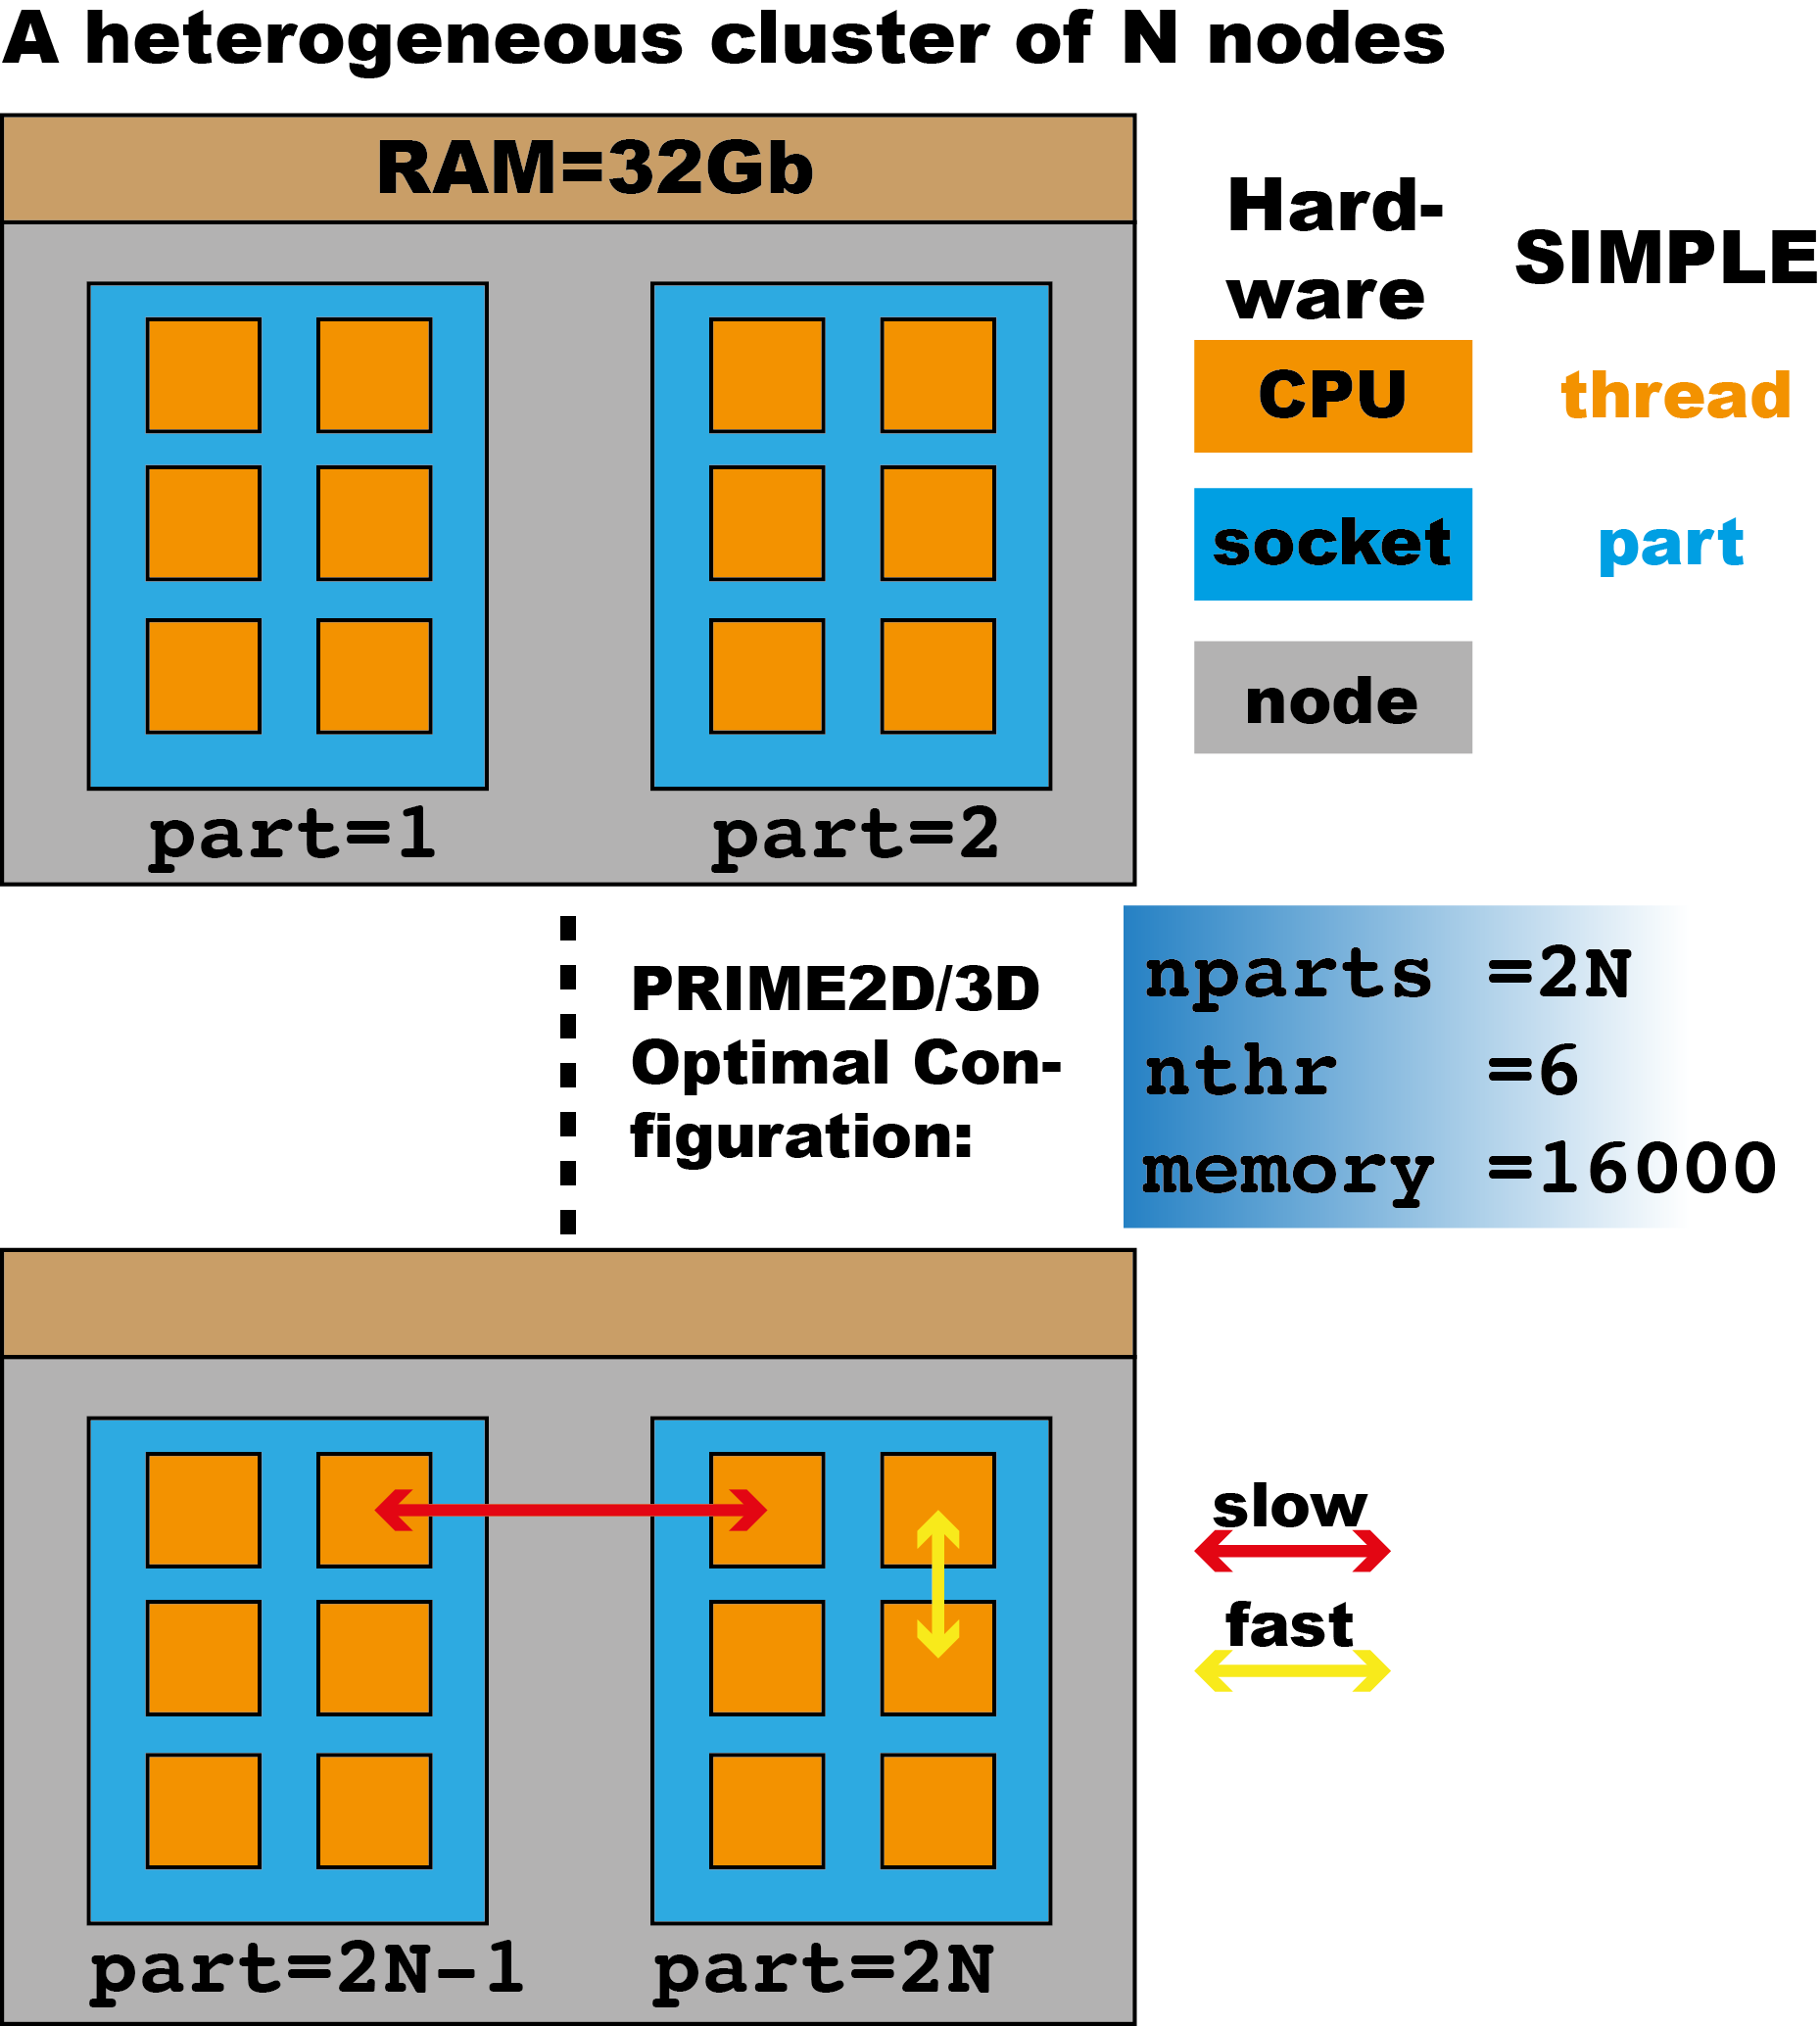
\includegraphics[keepaspectratio=true,scale=0.6]{../CPUtopo/cputopo}
\caption{\textbf{Configuration of the parallel PRIME-2D/3D execution on a heterogeneous cluster.} We here represent the nodes in  a heterogeneous cluster by two sockets with six CPUs each and 32Gb RAM/node. The best performance of PRIME--2D/3D is going to be obtained by partitioning  the jobs into \texttt{npart=2N} partitions, where \texttt{N} is the number of nodes. Each partition will then execute six threads \texttt{nthr=6} and these six threads will get access to half the RAM on the node (\texttt{memory=16000}) because we have two sockets per node that need to share the RAM between them}
\end{SCfigure}
If you are unsure how to configure your SIMPLE execution please file a help ticket.

We normally let \prgname{simple\_distr\_exec} run in the background on the login node of our cluster. An example of how to distribute \prgname{prime2D} using ten nodes is provided below.
\begin{Verbatim}[commandchars=+\[\],fontsize=\small,breaklines=true]
nohup simple_distr_exec prg=prime2D stk=ptcls.mrc smpd=1.77 msk=100
ncls=600 nthr=8 nparts=10 >> PRIME2DOUT &
\end{Verbatim}
Another option available on clusters that use the SLURM scheduler is to use the \texttt{srun} command for \prgname{simple\_distr\_exec} via
\begin{Verbatim}[commandchars=+\[\],fontsize=\small,breaklines=true]
srun --ntasks=1 --ntasks-per-socket=1 --cpus-per-task=1 --mem=32000 
--time=2-0:0:0 --output=PRIME2DOUT.%j --error=PRIME2DERR.%j
simple_distr_exec prg=prime2D stk=ptcls.mrc smpd=1.77 msk=100
ncls=600 nthr=8 nparts=10 &
\end{Verbatim}
However, beta testers have reported that srun job sometimes dies with no warning, possibly because of the low tolerance for network errors. A more robust route may be to use \texttt{sbatch} as follows
\begin{Verbatim}[commandchars=+\[\],fontsize=\small,breaklines=true]
sbatch -p MYCLUSTER --wrap="simple_distr_exec prg=prime2D stk=ptcls.mrc 
smpd=1.77 msk=100 ncls=600 nthr=8 nparts=10 >> PRIME2DOUT"
\end{Verbatim}
where the \texttt{--wrap} flag automatically generates a bash script for the given command.

\subsection{From Movies to Near-atomic Resolution Map}
These steps describe a typical SIMPLE workflow.
\begin{enumerate}
\item DDD (Direct Detector Device) movie alignment and frame-weighting using SIMPLE program \prgname{unblur}, executed with \texttt{simple\_distr\_exec}
\item CTF parameter identification with the SIMPLE program \prgname{ctffind}, wrapping CTFFIND4 \citep{rohou2015ctffind4}, executed with \texttt{simple\_distr\_exec}
\item Particle identification using EMAN2 \citep{Tang:2007aa} to generate \texttt{*.box} files
\item Particle extraction with SIMPLE program \prgname{extract}, executed with \texttt{simple\_exec}
\item 2D analysis using the SIMPLE \prgname{prime2D} distributed workflow, executed with \texttt{simple\_distr\_exec}
\item \textit{Ab initio} 3D reconstruction from class averages using the SIMPLE \prgname{ini3D\_from\_cavgs} distributed workflow, executed with \texttt{simple\_distr\_exec}
\item Mapping of class average selection and 3D class orientations to the particles using SIMPLE program \prgname{map2ptcls}, executed with \texttt{simple\_exec}
\item Reconstruction of a 3D map from the individual particle images with SIMPLE program \prgname{recvol}, executed with \texttt{simple\_distr\_exec}
\item Map refinement will be part of release 3.0
\end{enumerate}
For descriptions for how to execute the individual steps, please refer to the documentation of each program (below).

\subsection{Workflows for Analysis of Time-series data of Nanoparticles Spinning in Solution}
In addition to providing algorithms for analysis of electron microscopic projection images of biological molecules, SIMPLE also provides support for time-series analysis of nanoparticles spinning in solution.
\subsubsection{Time-series Pre-processing}
\begin{enumerate}
\item Convert the time-series from \texttt{*.dm4} format to the \texttt{*.mrc} format using the \prgname{dm42mrc.pl} script. This script assumes that you have \texttt{EMAN2} installed on your system.
\item Use the \prgname{tseries\_extract} program to generate overlapping windows of frames in the time series. We recommend a window size of 5. This program is executed via \texttt{simple\_exec prg=tseries\_extract}. The \texttt{frameavg} flag controls the size of the time-window.
\item Correct for stage drift and global beam-induced motion by processing the \texttt{*tseries\_frames*} stacks with \prgname{unblur}. It is important that you set \texttt{lpstart=5} and \texttt{lpstop=3} in addition to the required input parameters.
\item Use \texttt{EMAN1.9} or \texttt{EMAN2} to identify, in the first motion corrected frame, the particles that you want to track throughout the time-series. Write out a \texttt{*.box} file with the particle coordinates.
\item Use the \texttt{*.box} file created in the previous step in conjunction with the motion-corrected frames as input to the program \prgname{tseries\_track} to generate individual stacks of images representing the windowed nanoparticles as a function of time from the first to the last frame. Please execute \prgname{tseries\_track} using the \texttt{simple\_distr\_exec} binary. This will run the tracker in parallel mode with one CPU allocated per particle. The \texttt{ncunit} parameter controls the number of CPUs being used and this number cannot be larger than the number of particles to track in parallel.
Once the pre-processing workflow has been finalised, the problem becomes a standard single-particle reconstruction problem (one per particle stack). However, as SIMPLE was originally designed for biological single-particle EM image processing, there are a few parameter tuning strategies to consider (described below).
\end{enumerate}
\end{comment}

\def\bibfont{\footnotesize}
\bibliographystyle{cell}
\bibliography{Prime2bibfile}

\end{document}
